%%% The main file. It contains definitions of basic parameters and includes all other parts.

%% Settings for single-side (simplex) printing
% Margins: left 40mm, right 25mm, top and bottom 25mm
% (but beware, LaTeX adds 1in implicitly)
\documentclass[12pt,a4paper]{report}
\setlength\textwidth{145mm}
\setlength\textheight{247mm}
\setlength\oddsidemargin{15mm}
\setlength\evensidemargin{15mm}
\setlength\topmargin{0mm}
\setlength\headsep{0mm}
\setlength\headheight{0mm}
% \openright makes the following text appear on a right-hand page
\let\openright=\clearpage

%% Settings for two-sided (duplex) printing
% \documentclass[12pt,a4paper,twoside,openright]{report}
% \setlength\textwidth{145mm}
% \setlength\textheight{247mm}
% \setlength\oddsidemargin{14.2mm}
% \setlength\evensidemargin{0mm}
% \setlength\topmargin{0mm}
% \setlength\headsep{0mm}
% \setlength\headheight{0mm}
% \let\openright=\cleardoublepage

%% Character encoding: usually latin2, cp1250 or utf8:
\usepackage[utf8]{inputenc}

%% Further useful packages (included in most LaTeX distributions)
\usepackage{amsmath}        % extensions for typesetting of math
\usepackage{amsfonts}       % math fonts
\usepackage{amsthm}         % theorems, definitions, etc.
\usepackage{bbding}         % various symbols (squares, asterisks, scissors, ...)
\usepackage{bm}             % boldface symbols (\bm)
\usepackage{graphicx}       % embedding of pictures
\usepackage{fancyvrb}       % improved verbatim environment
\usepackage{natbib}         % citation style AUTHOR (YEAR), or AUTHOR [NUMBER]
\usepackage[nottoc]{tocbibind} % makes sure that bibliography and the lists
			    % of figures/tables are included in the table
			    % of contents
\usepackage{dcolumn}        % improved alignment of table columns
\usepackage{booktabs}       % improved horizontal lines in tables
\usepackage{paralist}       % improved enumerate and itemize
\usepackage[usenames]{xcolor}  % typesetting in color

%% my packages
\usepackage{algorithm}
\usepackage{algpseudocode}
\usepackage{mathtools}
\usepackage[acronym,toc]{glossaries}
\usepackage[toc,page,titletoc]{appendix}
\usepackage{dirtree}

\makeglossaries

%%% Basic information on the thesis

% Thesis title in English (exactly as in the formal assignment)
\def\ThesisTitle{Map-merging for multi-robot system}

% Author of the thesis
\def\ThesisAuthor{Jiří Hörner}

% Year when the thesis is submitted
\def\YearSubmitted{2016}

% Name of the department or institute, where the work was officially assigned
% (according to the Organizational Structure of MFF UK in English,
% or a full name of a department outside MFF)
\def\Department{Department of Theoretical Computer Science and Mathematical Logic}

% Is it a department (katedra), or an institute (ústav)?
\def\DeptType{Department}

% Thesis supervisor: name, surname and titles
\def\Supervisor{RNDr. David Obdržálek, Ph.D.}

% Supervisor's department (again according to Organizational structure of MFF)
\def\SupervisorsDepartment{Department of Theoretical Computer Science and Mathematical Logic}

% Study programme and specialization
\def\StudyProgramme{Computer Science}
\def\StudyBranch{General Computer Science}

% An optional dedication: you can thank whomever you wish (your supervisor,
% consultant, a person who lent the software, etc.)
\def\Dedication{%
Dedication.
}

% Abstract (recommended length around 80-200 words; this is not a copy of your thesis assignment!)
\def\Abstract{%
Abstract.
}

% 3 to 5 keywords (recommended), each enclosed in curly braces
\def\Keywords{%
{map-merging} {multi-robot system} {ROS} {SLAM} {computer vision}
}

%% The hyperref package for clickable links in PDF and also for storing
%% metadata to PDF (including the table of contents).
\usepackage[pdftex,unicode]{hyperref}   % Must follow all other packages
\hypersetup{breaklinks=true}
\hypersetup{pdftitle={\ThesisTitle}}
\hypersetup{pdfauthor={\ThesisAuthor}}
\hypersetup{pdfkeywords=\Keywords}
\hypersetup{urlcolor=blue}

% Definitions of macros (see description inside)
%%% This file contains definitions of various useful macros and environments %%%
%%% Please add more macros here instead of cluttering other files with them. %%%

%%% Minor tweaks of style

% These macros employ a little dirty trick to convince LaTeX to typeset
% chapter headings sanely, without lots of empty space above them.
% Feel free to ignore.
\makeatletter
\def\@makechapterhead#1{
  {\parindent \z@ \raggedright \normalfont
   \Huge\bfseries \thechapter. #1
   \par\nobreak
   \vskip 20\p@
}}
\def\@makeschapterhead#1{
  {\parindent \z@ \raggedright \normalfont
   \Huge\bfseries #1
   \par\nobreak
   \vskip 20\p@
}}
\makeatother

% This macro defines a chapter, which is not numbered, but is included
% in the table of contents.
\def\chapwithtoc#1{
\chapter*{#1}
\addcontentsline{toc}{chapter}{#1}
}

% Draw black "slugs" whenever a line overflows, so that we can spot it easily.
\overfullrule=1mm

%%% Macros for definitions, theorems, claims, examples, ... (requires amsthm package)

\theoremstyle{plain}
\newtheorem{thm}{Theorem}
\newtheorem{lemma}[thm]{Lemma}
\newtheorem{claim}[thm]{Claim}

\theoremstyle{plain}
\newtheorem{defn}{Definition}

\theoremstyle{remark}
\newtheorem*{cor}{Corollary}
\newtheorem*{rem}{Remark}
\newtheorem*{example}{Example}

%%% An environment for proofs

%%% FIXME %%% \newenvironment{proof}{
%%% FIXME %%%   \par\medskip\noindent
%%% FIXME %%%   \textit{Proof}.
%%% FIXME %%% }{
%%% FIXME %%% \newline
%%% FIXME %%% \rightline{$\square$}  % or \SquareCastShadowBottomRight from bbding package
%%% FIXME %%% }

%%% An environment for typesetting of program code and input/output
%%% of programs. (Requires the fancyvrb package -- fancy verbatim.)

\DefineVerbatimEnvironment{code}{Verbatim}{fontsize=\small, frame=single}

%%% The field of all real and natural numbers
\newcommand{\R}{\mathbb{R}}
\newcommand{\N}{\mathbb{N}}

%%% Useful operators for statistics and probability
\DeclareMathOperator{\pr}{\textsf{P}}
\DeclareMathOperator{\E}{\textsf{E}\,}
\DeclareMathOperator{\var}{\textrm{var}}
\DeclareMathOperator{\sd}{\textrm{sd}}

%%% Transposition of a vector/matrix
\newcommand{\T}[1]{#1^\top}

%%% Various math goodies
\newcommand{\goto}{\rightarrow}
\newcommand{\gotop}{\stackrel{P}{\longrightarrow}}
\newcommand{\maon}[1]{o(n^{#1})}
\newcommand{\abs}[1]{\left|{#1}\right|}
\newcommand{\dint}{\int_0^\tau\!\!\int_0^\tau}
\newcommand{\isqr}[1]{\frac{1}{\sqrt{#1}}}

%%% Various table goodies
\newcommand{\pulrad}[1]{\raisebox{1.5ex}[0pt]{#1}}
\newcommand{\mc}[1]{\multicolumn{1}{c}{#1}}

%%% My macros

\DeclareMathOperator{\rank}{rank}
\DeclareMathOperator{\sgn}{sgn}
\DeclareMathOperator{\trace}{trace}
\DeclareMathOperator{\conv}{conv}
%\DeclareMathOperator{\R}{\mathbb{R}}
\DeclareMathOperator{\bigO}{\mathcal{O}}
\DeclarePairedDelimiter{\ev}{\operatorname{E}[}{]}
\DeclarePairedDelimiter{\prob}{\operatorname{P}[}{]}
%\DeclarePairedDelimiter{\abs}{\lvert}{\rvert}
\DeclarePairedDelimiter{\ceil}{\lceil}{\rceil}
\DeclarePairedDelimiter{\floor}{\lfloor}{\rfloor}
\DeclarePairedDelimiter{\norm}{\lVert}{\rVert}
\DeclarePairedDelimiter{\scal}{\langle}{\rangle}

\renewcommand{\algorithmicrequire}{\textbf{Input:}}
\renewcommand{\algorithmicensure}{\textbf{Output:}}

% ROS node API formatting
\newcommand{\ROStopic}[3]{\begin{sloppypar} \noindent\texttt{#1} (#2) \end{sloppypar} \par \hangindent=15pt \hangafter=0 \noindent #3}
\newcommand{\ROSparam}[4]{\begin{sloppypar} \noindent\texttt{#1} (#3, default: \texttt{#2}) \end{sloppypar} \par \hangindent=15pt \hangafter=0 \noindent #4}
\newcommand{\ROStransform}[3]{\begin{sloppypar} \noindent\texttt{#1} $\rightarrow$ \texttt{#2} \end{sloppypar} \par \hangindent=15pt \hangafter=0 \noindent #3}

% allow hyphenation after underscore
\let\oldunderscore\_
\renewcommand{\_}{\oldunderscore\-}

\hyphenation{mer-ged}


% Definitions of acronyms
%%% Abbreviations used in the thesis, if any, including their explanation

\newacronym{RANSAC}{RANSAC}{random sample consensus}
\newacronym{BFS}{BFS}{breadth-first search}
\newacronym{DFS}{DFS}{depth-first search}
\newacronym{ROS}{ROS}{Robot Operating System}
\newacronym{OpenCV}{OpenCV}{Open Source Computer Vision Library}
\newacronym{ORB}{ORB}{Oriented FAST and Rotated BRIEF}
\newacronym{SIFT}{SIFT}{scale-invariant feature transform}
\newacronym{SURF}{SURF}{Speeded Up Robust Features}
\newacronym{SLAM}{SLAM}{simultaneous localization and mapping}
\newacronym{FLANN}{FLANN}{Fast Library for Approximate Nearest Neighbors}
\newacronym{SIG}{SIG}{Special Interest Group}


% Title page and various mandatory informational pages
\begin{document}
%%% Title page of the thesis and other mandatory pages

%%% Title page of the thesis

\pagestyle{empty}
\hypersetup{pageanchor=false}
\begin{center}

\large

Charles University in Prague

\medskip

Faculty of Mathematics and Physics

\vfill

{\bf\Large BACHELOR THESIS}

\vfill

\centerline{\mbox{
\includegraphics[width=60mm]{../img/logo.pdf}}}

\vfill
\vspace{5mm}

{\LARGE\ThesisAuthor}

\vspace{15mm}

{\LARGE\bfseries\ThesisTitle}

\vfill

\Department

\vfill

\begin{tabular}{rl}

Supervisor of the bachelor thesis: & \Supervisor \\
\noalign{\vspace{2mm}}
Study programme: & \StudyProgramme \\
\noalign{\vspace{2mm}}
Study branch: & \StudyBranch \\
\end{tabular}

\vfill

% Zde doplňte rok
Prague \YearSubmitted

\end{center}

\newpage

%%% Here should be a bound sheet included -- a signed copy of the "bachelor
%%% thesis assignment". This assignment is NOT a part of the electronic
%%% version of the thesis. DO NOT SCAN.

%%% A page with a solemn declaration to the bachelor thesis

\openright
\hypersetup{pageanchor=true}
\pagestyle{plain}
\pagenumbering{roman}
\vglue 0pt plus 1fill

\noindent
I declare that I carried out this bachelor thesis independently, and only with the cited
sources, literature and other professional sources.

\medskip\noindent
I understand that my work relates to the rights and obligations under the Act No.~121/2000 Sb.,
the Copyright Act, as amended, in particular the fact that the Charles
University in Prague has the right to conclude a license agreement on the use of this
work as a school work pursuant to Section 60 subsection 1 of the Copyright Act.

\vspace{10mm}

\hbox{\hbox to 0.5\hsize{%
In ........ date ............	% FIXME!
\hss}\hbox to 0.5\hsize{%
signature of the author
\hss}}

\vspace{20mm}
\newpage

%%% Mandatory information page of the thesis

\openright

\vbox to 0.5\vsize{
\setlength\parindent{0mm}
\setlength\parskip{5mm}

Title:
\ThesisTitle

Author:
\ThesisAuthor

\DeptType:
\Department

Supervisor:
\Supervisor, \SupervisorsDepartment

Abstract:
\Abstract

Keywords:
\Keywords

\vss}

\newpage

%%% Dedication

\openright

\noindent
\Dedication

\newpage

\openright
\pagestyle{plain}
\pagenumbering{arabic}
\setcounter{page}{1}


%%% A page with automatically generated table of contents of the bachelor thesis

\tableofcontents

%%% Each chapter is kept in a separate file
\chapwithtoc{Introduction}

Multi-robot exploring teams have several advantages over a single robot. When properly coordinated performace of the multi-robot system is higher, single point of failure can be eliminated and multiple robots can possibly do tasks single robot could not.

Multi-robot systems are not limited to exploration tasks, applications include: payloads delivery, military tasks, search and rescue in disaster areas and patroling. Multi-robot teams can overcome imperfections in underlying navigation and mapping algorithms especially when using heterogeneous robot teams, where stucked robot can be replaced by robot which uses different algorithm.

In multi-robot systems shared map is required for effective coordination. Map-merging algorithm producing global map is therefore essential component of multi-robot systems. Map-merging is a challenging problem, especially in heterogeneous systems.

Key aspects of map-merging and related works are discussed in section~\ref{chap:map-merging-intro}. In section~\ref{chap:mergingalgorithm} I present a novel map-merging algorithm based on image stitching techniques, which can work with heterogeneous multi-robot teams and is scalable to large number of robots.

Section~\ref{chap:ros-packages} presents ready-to-use \gls{ROS} packages implementing presented map-merging algorithm and frontier-based autonomous exploration. Section~\ref{chap:evaluation} discusses performace of presented map-merging algorithm achieved in several simulation experiments.

Documentation for \gls{ROS} packages presented in section~\ref{chap:ros-packages} is attached as appendices~\ref{chap:map_merge-doc}, \ref{chap:explore-doc}.

\chapter{Initial pose estimation problem}
\label{chap:map-merging-intro}

Key problem of map-merging is getting transformation between reference frames of robots. When the transformation is known, merging maps produced by robots is simple. In such a case we can compute transformation to chosen global reference frame and overlay maps in global reference frame. Errors in maps especially while mapping in dynamic environment may lead to different values across maps for specific global frame coordinates, but this can be solved by taking arithmetic mean, median or extremal values for such coordinates.

Transformation between grids can be acquired from initial poses of robots and vice versa, considering initial pose is represented as origin in the map (or generally any fixed point). This holds usually true for existing implementations of \gls{SLAM} algorithms.

Problem arises when initial poses of robots are not known to merging algorithm. When robots are starting from the same place, initial relative positions can be measured with basic equipment either present on the site or mounted on robots. When robots are starting from distant locations measuring initial poses might require more sophisticated equipment, as widely available hardware such as \gls{GPS} sensors might not provide required precision. In indoor environments determining starting positions might be even more challenging.

Because of these difficulties, algorithms that can estimate transformations between maps and then merge maps without knowledge of initial positions have been developed. A comprehensive survey of map-merging techniques is done in~\cite{Lee2012}, which classifies algorithms as Direct Map Merging and Indirect Map Merging.

\section{Direct map merging}

Direct map-merging algorithm relies on sensors to directly compute transformation between reference frame of robots. This includes techniques relying on direct robot rendezvous~\cite{Zhou2006} and similar. This techniques can provide a highly accurate transformation estimate, but are limited by relying on specific conditions to estimate this transformation such as the robot rendezvous or encountering specific landmark. These systems also exchange specific data related to selected feature or sensor to estimate transformation; some algorithms even require control over robot such as solution presented in~\cite{Konolige2003}. Implementations therefore tend to be monolithic, because they rely on exchange of custom messages and specific sensors data, which makes them hard to implement especially for heterogeneous robots.

\section{Indirect map merging}
\label{sec:indirect-map-merging}

Indirect map-merging algorithms use overlapping areas in maps to estimate transformation between maps. Merging maps based on map data only naturally creates a common interface and works well for heterogeneous groups of robots. Each robot is only required to expose its map in a common format, sensor equipment mounted on robots may be different as well as a \gls{SLAM} algorithm used for creating the map. This makes indirect map-merging algorithms more flexible than direct map merging: robots may visit overlapping area at different times (in contrast to robot rendezvous) and this approach is also absolutely passive requiring no control over robot.

Wide range of techniques has been employed for indirect map merging. \cite{Lee2012} mentioned in this category techniques based on scan matching algorithms. These algorithms are working with \gls{SLAM} representation of maps and they are usually tightly coupled with specific \gls{SLAM} algorithm. This makes them share some disadvantages (such as difficult scalability through heterogeneous systems) with direct map merging algorithms. Algorithms in this category include \cite{Wang2012} work based on visual \gls{SIFT} features and topology nodes, approach of~\cite{Tungandi2010} combining omnidirectional vision and laser scans, \cite{Cunningham2012} using graph \gls{SLAM} with condensed maps and non-linear constrained optimization to acquire transformation between maps. Data used by the \gls{SLAM} algorithm to represent map may be too big to exchange all of them between robots, this was addressed in the work by~\cite{Lazaro2013}, which uses condensed measurements and multi-robot graph \gls{SLAM}.

Only a few algorithms works exclusively with portable map representation (maps represented as two-dimensional occupancy grids), despite this promises better scalability and by design supports heterogeneous multi-robot systems. Works using occupancy grids include spectra-based approach of~\cite{Carpin2008}. \cite{Lee2011} combines his approach with concept of virtual supporting lines to merge custom sparse maps of infrared features. \cite{martins2013mrslam} used algorithm of~\cite{MapstitchROS} based on image features to merge maps of $2$ robots, which is limitation of this algorithm.

The novel algorithm for map merging presented in section~\ref{chap:mergingalgorithm} is using only occupancy grids to produce the merged map. This algorithm is inspired by image stitching algorithms for creating photo panoramas. It is designed to merge maps from arbitrary number of robots, overcoming the limitation of both~\cite{MapstitchROS} and \cite{Carpin2008}. It employs \gls{RANSAC} for robust transform estimation and uses probability model to evaluate confidence of estimated transformation. Matching phase is accelerated using parallel hierarchical clustering trees proposed by~\cite{Muja2012} so that algorithm scales well to large number of robots.

% http://journals.cambridge.org/article_S026357471100049X

\chapter{Merging algorithm}
\label{chap:mergingalgorithm}

In this chapter we present an merging algorithm for two-dimensional feature map-merging based on computer vision techniques. This is not completely new even in \gls{ROS} environment. First computer vision-based approach to merging was implemented in~\cite{MapstitchROS}. This package's primary purpose was to stitch generated map to existing static map.

Although this package was not developed for map merging in multi-robot configuration, algorithm and its original implementation were used for coordinated multi-robot exploration solution presented in~\cite{Andre2014}.

Due to its original purpose, mapstitch algorithm shows some limitations for multi-robot map merging setup. Originally it was designed for offline use~\cite{Andre2014}. Also, it was designed for stitching two maps, one them being large reference map covering most of the environment. Although it is possible to incrementally merge maps from multiple robots with this algorithm, global map quality generally decreases with increasing number of robots. Significant decrease in performance was observed for 4 robots~\cite{Andre2014}.

\begin{algorithm}
    \caption{Mapstitch original algorithm}
    \label{alg:mapstitch}
    \begin{algorithmic}[1]
        \Require $2$ occupancy grids
        \Ensure transformation between $2$ grids
        \Procedure{StitchedMap}{$grid1, grid2$}
            \State detect \gls{ORB} features
            \State match keypoints with Brute-Force matcher
            \State find matching point pairs with same distance in both images
            \State find homography (affine transform)
        \EndProcedure
    \end{algorithmic}
\end{algorithm}

Algorithm~\ref{alg:mapstitch} shows original algorithm used in~\cite{MapstitchROS}, version used in~\cite{Andre2014} is only a slightly modified.

Although our algorithm also uses computer vision-based approach, proposed algorithm deals with most of the limitations of the original simple algorithm. Proposed algorithm is designed to work with unlimited number of grids, so there is no additional need for iterative merging. More importantly, by design, algorithm can determine optimal order of individual pairwise merges. I assume this might be the main reason for decrease in performance in $4$-robot setup observed by~\cite{Andre2014}. Also proposed algorithm deals with other problems arising for general $n$-map merge problem such as situations when it is not possible to merge some of the maps because transformation to others could not be reliably estimated, cases where map transformation can be estimated from more sources (multiple neighbours) etc.

\section{Stitching pipeline} % (fold)
\label{sec:stitchingpipeline}

As discussed in chapter \#reference here\# our algorithm is inspired by image stitching algorithms. Stitching algorithms are well-understood and implementations are broadly available. General concept of multi-step stitching pipeline is described in~\cite{Brown2006}. Stitching pipeline is also well established code in \gls{OpenCV}, mostly based on~\cite{Brown2006}, along with~\cite{Szeliski2004} \cite{Shum1998} and others. Figure~\ref{fig:opencv} highlights processing steps in stitching as implemented in \gls{OpenCV}.

\begin{figure}
	\centering
	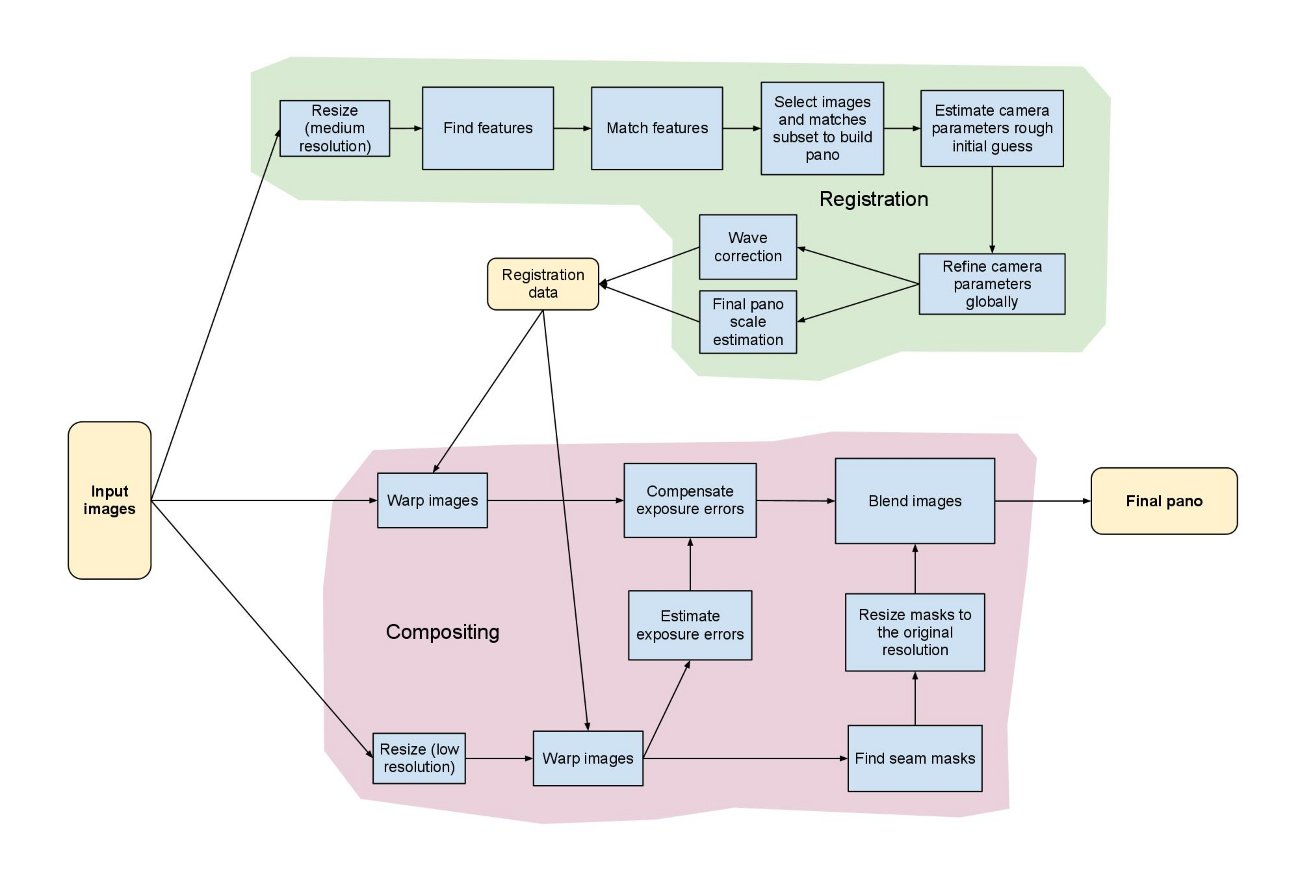
\includegraphics[width=4.33in]{../img/StitchingPipeline.jpg}
	\caption{\gls{OpenCV} Stitching pipeline.}
	\label{fig:opencv}
\end{figure}

Our algorithm will solve the registration part of stitching according to figure~\ref{fig:opencv}. As compositing part of stitching is relatively simple for occupancy grids compared to images from camera, because we don't need to compensate exposure errors, gain and other deficiencies. This solves the main problem of acquiring transformation between robots individual frames and bridging the problem of merging maps with known initial positions and unknown initial positions.

\gls{ROS} node for map merging described in \#reference here\# implements also compositing part of the pipeline, which is simple when transformation is estimated with high precision.

For description of the algorithm we will assume to have maps represented as occupancy grids, with each cell containing value in range $[0,100]$ indicating probability that there is obstacle in the cell and $-1$ for indicating unknown probability. This representation is basically greyscale image, hence using image processing algorithms seems natural.

We will consider occupancy grids greyscale images through algorithm~\ref{alg:estimategridtrasform}. Values in the image are exactly the same is in occupancy grids, without any mapping. This means images are be basically only $7$-bit depth.

Algorithm~\ref{alg:estimategridtrasform} offers overview of the proposed algorithm, detailed description will be provided in following sections.

\begin{algorithm}
    \caption{Proposed algorithm for estimating transform between multiple occupancy grids}
    \label{alg:estimategridtrasform}
    \begin{algorithmic}[1]
        \Require occupancy grids
        \Ensure for each grid: transformation between grid and global reference frame, or value indicating transformation could not be be estimated for current grid
        \Procedure{estimateGridTransform}{$grids$}
            \State detect \gls{ORB} features (keypoints) for each grid
            \ForAll{pair of grids} \Comment{we will compute transformation between each image along with confidence}
            	\State match features
            	\State $n \gets \text{number of matches}$
            	\If{$n \le \text{matches threshold}$}
            		\State confidence $\gets 0$
            	\Else
            		\State find restricted affine transformation for keypoints using \gls{RANSAC}
            		\State $\psi \gets \text{number of inliers in \gls{RANSAC}}$
            		\If{transformation found}
            			\State confidence $\gets \frac{\psi}{8 + 0.3 \cdot n}$
            		\Else
            			\State confidence $\gets 0$
            		\EndIf
            	\EndIf
            \EndFor
            \State matches $\gets (i,j)$ for matches with confidence $\ge 1.0$
            \State $g \gets (grids, matches)$
            \State $h \gets$ largest connected component in $g$
            \State $t \gets$ maximum spanning tree in $h$
            \State walk $t$ and compute transformations to global reference frame
        \EndProcedure
    \end{algorithmic}
\end{algorithm}

% section stitching_pipeline (end)

\section{Feature detection} % (fold)
\label{sec:featuredetection}

Stitching pipeline proposed in \cite{Brown2006} is using \gls{SIFT} features. \gls{SIFT} features have been used with success for stitching in many applications. Some of the recent approaches to stitching, improving traditional \gls{SIFT}-based algorithm, are also building on top of \gls{SIFT} features \cite{Xie2015}. \gls{SIFT} features are patented in the US \cite{lowe2004method}, limiting its use.

I have decided to use \gls{ORB} as feature detector a descriptor described in \cite{Rublee2011}. \gls{ORB} algorithm is patent-free, and available in \gls{OpenCV}. \gls{ORB} features has been already used with occupancy grid images \cite{MapstitchROS} \cite{Andre2014}.

Other alternatives for feature detection and feature description has not been tested yet. Performance of other detectors for map merging and effect of choose of detector to overall merging performance remains to be evaluated. Some feature detectors and descriptors promising good performance are \cite{Alahi2012} \cite{alcantarilla2011fast} \cite{calonder2010brief}.

For image stitching, images are usually downscaled for further processing as seen is figure~\ref{fig:opencv}. Feature extraction and feature matching on smaller images is considerably faster and final performance is acceptable. I don't propose any such down scaling for occupancy grids. Occupancy grids acquired from mapping are usually smaller than multi-megapixel images from camera, so stitching time is reasonable even for full-scale grids. Also occupancy grids have usually much smaller number of features than photos making stitching harder and less precise.

During online merging we can run stitching with low frequency even if higher map update frequencies are required by simply using previously estimated transform between grids. This further reduces cost of estimation over time. Since transformation between grids is fixed in most cases (when \gls{SLAM} algorithm work reasonably well), depending only on starting points of robots, this approach does not reduce map quality considerably.

In most tested scenarios estimated transformation change only during initial phase. After there is enough overlapping regions in the map, such that transformation can be estimated with enough precision, transformation estimated with stitching algorithm remains stable over time. This property allows to run re-estimation with low frequencies.

% section feature_detection (end)

\section{Pairwise matching} % (fold)
\label{sec:pairwisematching}

Pairwise matching is the most resource demanding part of the algorithm. We do matching for all $\bigO(n^2)$ pairs of grids. For panorama images it is possible to push this down to $\bigO(n)$ matching by expecting photos to be taken in ordered sequence. We can then match image only $k$ neighbours (for small $k$) in sequence, because neighbours are expected to have overlapping area.

For occupancy grids in multi-robot mapping scenario it is impractical to assume any such ordering in robot's initial poses. It might not even be possible when robots are exploring given areas independently. Our algorithm therefore always match all $\bigO(n^2)$ pairs.

Because computations in each pair are independent it is easy to run matching of all pairs in parallel or offload it GPU. This approach is used in map merging node presented in \#reference here\#.

\begin{figure}
    \centering
    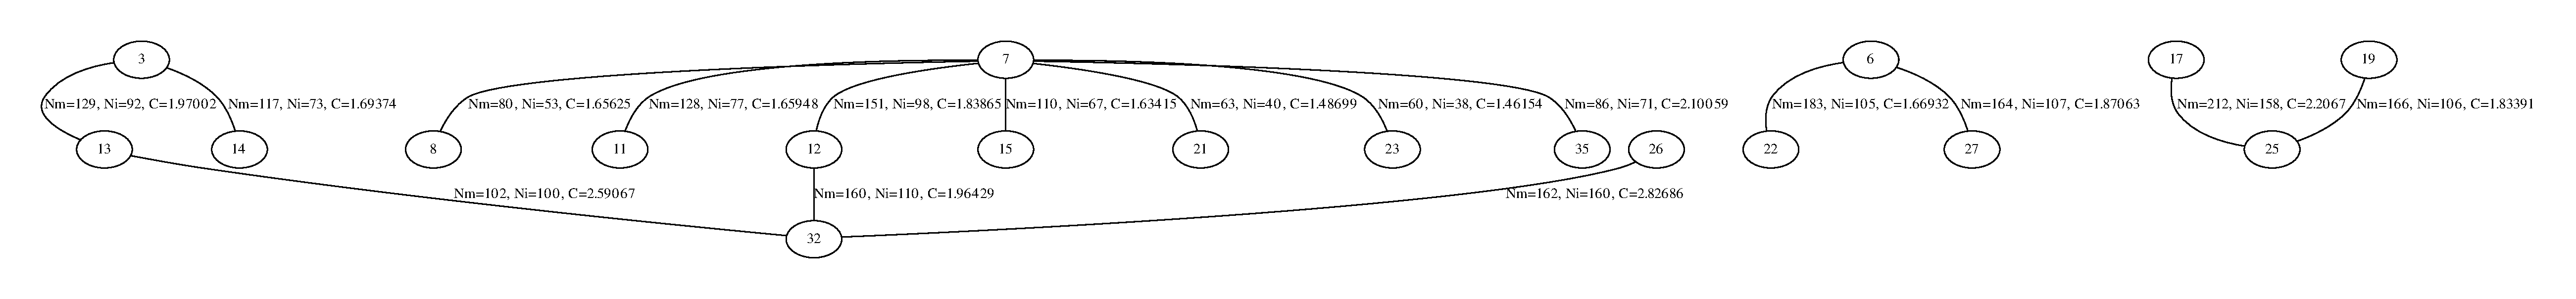
\includegraphics[width=\textwidth]{../img/matches.pdf}
    \caption{Graph showing matches between $37$ occupancy grids during map merging. This graph was acquired for maps from MIT dataset, see chapter \#reference here\#. Grids without any matches are omitted. Legend: $Nm$ number of matches, $Ni$ number of inliers from \gls{RANSAC}, $C$ confidence.}
    \label{fig:matches}
\end{figure}

Figure~\ref{fig:matches} shows matching results for $37$ occupancy grids acquired during experiment \#reference here\#.

Because of non-linear number of pairs it is usually too computationally expensive to search for matches using simple (brute-force) search unless this can be offloaded to GPU. For matching on CPU it is better to use approximate methods, which can be much faster.

For vector-based features, such as \gls{SIFT} and \gls{SURF}, the solution has been to use approximate nearest-neighbour search, but these existing algorithms are not suitable for binary features \cite{Muja2012}. For \gls{ORB} features, which are binary based, searching for nearest neighbours using parallel hierarchical clustering trees proposed in \cite{Muja2012} can provide similar speed-up for \gls{ORB} features. This method is used through the \gls{FLANN} by the same authors, which is now part of \gls{OpenCV}.

When matching keypoints are found for pair of grids, algorithm estimates transformation between grids. Traditional image stitching algorithms are using homography in projective spaces, which is a good for modelling perspective affecting camera images. For occupancy grids this is not an expected transformation under normal circumstances, and even when there are errors in maps produced by \gls{SLAM} algorithm, these are not errors produced by projective transformation.

For occupancy grids we propose a different model based on reduced affine transform. This is a partial affine transformation with $4$ degrees of freedom.

\begin{defn}[Reduced affine transformation]
For given matrices $R$ (rotation), $S$ (scaling), $T$ (translation), where

\begin{align}
    R &=
    \begin{pmatrix}
        \cos{\theta} & -\sin{\theta} \\
        \sin{\theta} & \cos{\theta} \\
    \end{pmatrix} \\
    S &=
    \begin{pmatrix}
        s & 0 \\
        0 & s \\
    \end{pmatrix} \\
    T &=
    \begin{pmatrix}
        tx \\
        ty \\
    \end{pmatrix}
\end{align}

we define matrix of reduced affine transformation as

\begin{equation}
    A =
    \begin{pmatrix}
        RS|T
    \end{pmatrix}
    =
    \begin{pmatrix}
        \cos(\theta)s & -\sin(\theta)s & tx \\
        \sin(\theta)s & \cos(\theta)s & ty \\
    \end{pmatrix}
\end{equation}.
\end{defn}

As usual when representing translations we will work with reduced affine transformation in homogeneous coordinates, where this transformation is homomorphism. Therefore we extend $A$ as

\begin{equation}
    A' =
    \begin{pmatrix}
        \cos(\theta)s & -\sin(\theta)s & tx \\
        \sin(\theta)s & \cos(\theta)s & ty \\
        0 & 0 & 1 \\
    \end{pmatrix}
\end{equation}

to represent reduced affine transformation in homogeneous coordinates space.

For pair of matched points $X=\T{(x_1,x_2,1)}$, $Y=\T{(y_1, y_2, 1)}$ we can then solve

\begin{align}
    A'X &= Y \label{eq:affinetrans}\\
    \begin{pmatrix}
        \cos(\theta)s & -\sin(\theta)s & tx \\
        \sin(\theta)s & \cos(\theta)s & ty \\
        0 & 0 & 1 \\
    \end{pmatrix}
    \begin{pmatrix}
        x_1 \\
        x_2 \\
        1
    \end{pmatrix}
    &=
    \begin{pmatrix}
        y_1 \\
        y_2 \\
        1
    \end{pmatrix}
\end{align}

for $\T{(\cos(\theta)s, \sin(\theta)s, tx, ty)}$ to obtain transformation between grids. This is easy to solve and need only $2$ points to get the transformation.

Reduced affine transformation is chosen to model transformation between initial robot poses in $2D$ space. Each robot can start at different position and have different orientation in terms of rotation in $2D$ space. Scaling enables occupancy grids to have different resolution.

We combine~\eqref{eq:affinetrans} with \gls{RANSAC}~\cite{fischler1981random} method to obtain final transformation. \gls{RANSAC} is used to estimate homography in image stitching method proposed in~\cite{Brown2006}. We use the same method for estimating reduced affine transformation. Using \gls{RANSAC} has another advantage. We can used number of inliers in \gls{RANSAC} to estimate transformation accuracy.

For each pair we compute confidence as $\frac{\psi}{8 + 0.3 \cdot n}$, where $n$ is number of matches and $\psi$ is number of inliers in \gls{RANSAC}. Model for confidence is based on probabilistic model for image match verification proposed in~\cite{Brown2006}.

For \gls{RANSAC} I have chosen following parameters: maximum number of iterations $500$, good ratio $0.5$. Same parameters are used internally in \gls{OpenCV}. If maximum number of iteration is reached and transformation therefore could not be found, its confidence is set to $0$.

% section pairwise_matching (end)

\section{Finding largest connected component} % (fold)
\label{sec:findinglargestconnectedcomponent}

As seen in figure~\ref{fig:matches} it is common that not all transformations could be established between grids. Graph of matchings therefore can have multiple connected components. We need to deal with missing transformations between components to estimate transformations for grids.

We could include all components to resulting map and position them such they don't overlap. This setup would preserve all information, but resulting map can't be topologically correct. Another approach is to choose only one connected component for final merge. This approach preserves map's topological accuracy. I have chosen the latter approach.

As a next in the algorithm we filter out matches according to selected probabilistic model for accuracy. Matches with computed confidence $\le 1.0$ are not further considered for matching.

After matches are filtered largest component is found in matches graph. Transformation will be established only for grids in largest connected component.

Choosing largest connected component might seem natural, but this approach has its caveats. Largest connected component represents matches between largest number of robots, however maps from the largest number of robots does not need to represent largest area in the map. This might be a problem especially in systems with heterogeneous robots, where mapping performance differs greatly between robots. Also some parts of maps might be much harder for robots to explore and despite large number of robots in such an area, produced map may be smaller than map produced by other group of robots (represented in graph as smaller component).

Modifications of this algorithm might choose to find weighted largest connected component in matchings graph. Weight could be based on discovered area in each map, such that the largest weighted connected component would represent largest discovered area.

I have chosen to use unweighted largest connected component, because it is less computationally expensive (weighting grids to represent discovered area in each grid require visiting each cell of each grid). Algorithm using unweighted largest connected component provides good results for small number of robots \#reference here\#. Approach using weighted components needs to be evaluated for more robots and larger environments.

% section finding_largest_connected_component (end)

\section{Estimate final transformation} % (fold)
\label{sec:estimatefinaltransformation}

Remaining graph is connected and it is possible to estimate transformation for all grids. We have estimated transformations between pairs of grids, edges for some pairs may be missing, because they were filtered out in previous steps.

Final part of the algorithm estimates transformation to global reference frame for each grid. We can choose reference frame of one of the grids as global reference frame, because we are interested in relative transformations between all grids for merging. This will be the reference frame of merged map.

Selecting global reference frame is not enough, because there may exist multiple paths from grid selected as reference frame to other grids. We construct maximum spanning tree to break these cycles. Edges are weighted with number of inliers to prefer stronger matches. This approach is routinely used for image stitching, exactly the same construct is implemented in \gls{OpenCV}.

Finally we can walk through spanning tree to obtain final transforms. There is now only one path from grid selected as reference frame to other grids. For each grid we can get the final by compositing pairwise transformations along the path. As we are working in homogeneous coordinates this is equivalent to matrix product of pairwise transformations along the path. This can be done in linear time with algorithm~\ref{alg:estimatefinaltrans}.

\begin{algorithm}
    \caption{Algorithm estimating transformations to global reference frame from pairwise transformations on spanning tree.}
    \label{alg:estimatefinaltrans}
    \begin{algorithmic}[1]
        \Require $t$ maximum spanning tree on grids, $P_{(i,j)}$ is pairwise reduced affine transformation between grids $i, j$
        \Ensure $T_i \forall i \in V$ transformations
        \Procedure{estimateFinalTrasform}{$t = (V,E)$, $P_e \forall e \in e$}
            \State $e \gets$ edges of $t$ sorted by discover time in \gls{BFS} started from grid with reference frame \Comment{using \gls{BFS} or \gls{DFS} does not matter here}
            \State $\forall T_i: T_i \gets I$ \Comment{initialize transformations with identity}
            \ForAll{$(i,j)$ in $e$}
                $T_j \gets T_i P_{(i,j)}$
            \EndFor
        \EndProcedure
    \end{algorithmic}
\end{algorithm}

% section estimate_final_transformation (end)
\chapter{ROS packages}
\label{chap:ros-packages}

It this section I present \gls{ROS} packages developed as part of this work. Merging algorithm presented in Section~\ref{chap:mergingalgorithm} was implemented in \gls{ROS} package \texttt{multirobot\_map\_merge}. To evaluate performance of map-merging in multi-robot exploring scenarios I have developed the second package, \texttt{explore\_lite} for autonomous exploring.

Both packages are now part of the \gls{ROS} distribution. Documentation for packages is available online at the \gls{ROS} wiki pages:

\begin{itemize}
	\item \url{http://wiki.ros.org/multirobot_map_merge}
	\item \url{http://wiki.ros.org/explore_lite}
\end{itemize}

This documentation is also reproduced as Appendix~\ref{chap:map_merge-doc} and Appendix~\ref{chap:explore-doc}.

\section{\texttt{multirobot\_map\_merge} package} % (fold)
\label{sec:map_merge-package}

\texttt{multirobot\_map\_merge} package solves several problems for merging maps from multiple robots. Dynamic robot discovery, initial poses estimation and map composition.

Dynamic robot discovery allows efficient easy-to-use auto-configuration of the package and also allows number of robots to change during exploring. This design allows robots to be launched and assigned to system based on exploration progress.

Initial poses estimation is the key feature of this package allowing merging maps for robots with unknown initial positions. For situations where robots initial positions are known (simulations) or can be measured with required precision (required equipment is available on robots or at the starting place) \texttt{multirobot\_map\_merge} package supports merging with user-provided initial robots positions. This was also used for producing a reference map to evaluate performance of estimation algorithm.

Regardless of how transformation between grids have been acquired (from user supplied initial poses or estimated by the algorithm) map composition is the final step to produce a merged map. This phase must be able to deal with different map sizes between robots, different map resolutions and be able to apply scaling, rotation and translation transformations.

\subsection{Inter-robot communication}

Running map-merging for multiple physical robots requires network connection between robots. Managing this connection is deliberately out-of-scope of this package. However, solutions exists in \gls{ROS} to make this task relatively easy.

First of all \gls{ROS} is designed to work natively across multiple computers. This setup requires almost no configuration and is supported by default. In this configuration one of the computers/robots runs a \texttt{roscore} service (also referred as \gls{ROS} master), which acts as a directory listing (broker) service. All \gls{ROS} topics and \gls{ROS} services are available transparently through the whole network.

Main disadvantage of this setup is a single-point-of-failure \texttt{roscore} service. Although the communication in the \gls{ROS} network is always peer-to-peer, \texttt{roscore} is required for advertisement, enumerating topics and establishing communication. This might not be acceptable for exploration robots communicating over unreliable link.

\gls{ROS} community is aware that single \gls{ROS} master is a limiting factor for many applications. There is a \gls{ROS} Multi-master \gls{SIG}~\cite{MultiMasterSIG} coordinating efforts for multi-master support.

As part of these efforts there exists the \texttt{multimaster\_fkie} package, described in technical report~\cite{herrero2015multimaster}, which allows setting a multi-master network transparently.

\texttt{multirobot\_map\_merge} can work transparently with both configurations as it is not tied to any particular communication between robots, allowing a great flexibility. It can take an advantage of native \gls{ROS} communication in environments with reliable network link (such as a simulation running on a cluster) and use a user provided communication (such as the \texttt{multimaster\_fkie} package) for exploring harsh environments with unrelible link. This is an important difference to framework presented in~\cite{Andre2014}, which always depends on custom ad-hoc messaging.

\subsection{Dynamic robot discovery}

This package allows merging maps from arbitrary number of robots. To make configuration of map-merging easy, robots are auto-discovered during the merging procedure. This also allows robots to be added or removed during exploring.

This package requires only maps produced by \gls{SLAM} and does not depend on any additional info about robots. Robot discovery is implemented by scanning available \gls{ROS} map topics, each map topic is being considered as one robot (one map to be added for merging). This approach is inspired by a discovery algorithm introduced in~\cite{Yan2014}.

Robot discovery runs in parallel to map-merging at rate which is configurable. Robot discovery therefore does not negatively impacts map-merging performance, when configured at low rate.

\subsection{Initial poses estimation}

Initial poses estimation is necessary for situations where initial robot positions could not be measured with required precision by user. Package uses algorithm discussed in Section~\ref{chap:mergingalgorithm}, which was specifically designed for this purpose. When robots are starting from different places, getting the initial positions might be difficult without proper equipment. Even when robots are starting exploration from common place, it might be more comfortable for users to let merging system estimate initial positions itself. In this situation merging algorithm can take the advantage of initial overlapping area and produce high-quality merges quickly.

Estimation is designed to run in parallel to other parts of this package. Estimation rate is user-settable.

\subsection{Map composition}
\label{sec:map-composition}

After estimating transformation between grids, map composition combines final merged map. For map-merging task I have adapted the relevant code from \texttt{occu\-pan\-cy\_grid\_uti\-ls} package~\cite{Marthi2014}. This package is no longer available in current \gls{ROS} distribution, current version is maintained by Clearpath Robotics in github repository~\cite{GitHubOccGridUtils}. I have contributed some fixes to this repository, but as the code of \texttt{occu\-pan\-cy\_grid\_uti\-ls} is mostly obsolete in current \gls{ROS} distribution (most of the functionality is provided by \gls{ROS} navigation stack), I have decided to incorporate merging-related code directly to \texttt{multi\-robot\_map\_merge} package.

The code is robust, it can deal with all differences in size and resolution to allow merging maps in heterogeneous systems. This code however does not provide expected performance for merging big maps from large number of robots. In future versions of \texttt{multi\-rob\-ot\_map\_merge}, this algorithm may be changed for more efficient one.
Current solution works well for smaller groups of robots (up to $10$ robots) on low end hardware.

Merging frequency is user-adjustable and can be increased to deliver faster update frequency.
% section map_merge-package (end)

\section{\texttt{explore\_lite} package} % (fold)
\label{sec:explore_lite-package}

\texttt{explore\_lite} package provides \gls{ROS} node for autonomous exploration. Although there exists \gls{ROS} packages for exploring~\cite{2013:RoboCup}, \cite{DuHadway2010}, \cite{Bovbel2010} and exploring node from~\cite{Andre2014}, none of the existing packages met my requirements out-of-the-box. \cite{2013:RoboCup} is complex and includes custom navigation stack, \cite{DuHadway2010}, \cite{Bovbel2010} are not available as of Apr 2016 for current version of \gls{ROS} and \cite{Andre2014} offers some multi-robot coordination capabilities, but relies on custom ad-hoc communication between robots, which is an approach different from the map-merging node presented in Section~\ref{sec:map_merge-package}.

For purposes of evaluation of the presented map-merging node, I have developed a new exploration node for \gls{ROS}. This node is based on code of~\cite{DuHadway2010} with major improvements. Main design goal of this node is light-weightiness. I have needed to allow running more robots in a testing environment with limited resources. Although the node does not have multi-robot coordination capabilities as this was not required for running selected simulation scenarios, this node must handle properly \gls{ROS} namespaces and \texttt{tf} namespaces to allow running multiple robots under the same \gls{ROS} master. As a result of these requirements major parts of the node have been redesigned.

\subsection{Navigation}

\texttt{explore\_lite} uses \gls{ROS} standard stack for navigation through the \texttt{move\_base} node. The same approach is used by~\cite{DuHadway2010}, \cite{Bovbel2010} and \cite{Andre2014}.

\subsection{Map sourcing}
\label{sec:map-sourcing}

Exploring packages, which use the \gls{ROS} navigation stack~\cite{Bovbel2010} and \cite{DuHadway2010} are using a local costmap provided by \gls{ROS} navigation packages through \texttt{Cost\-map\-2D\-ROS}. The local costmap is then used to search for frontiers and finding paths to frontiers from the robot's position.

\texttt{Costmap2DROS} is a feature-rich framework for building costmaps, allowing usage of plugins and several layers for costmaps. It can build costmaps from various sources including laser scans and handle inflating obstacles on-the-fly. Although all these features are great when building a costmap for robot navigation purposes it brings an unnecessary overhead when using the costmap for searching for frontiers and other exploration purposes.

For the \texttt{explore\_lite} package I have introduced a custom \texttt{costmap\_client} code, which subscribes to a map source in the \gls{ROS} and provides a local costmap with only minimal processing. This reduces the overhead significantly compared to the situation when the costmap is build by ray-tracing from scans in explore node. Provided local costmap is then used for both frontier search and planing.

Choosing the right map source can also improve frontier discovery accuracy. Constantly better results has been achieved when the local costmap has been built from \gls{SLAM}-constructed map, instead of a laser ray-traced costmap, such as the costmap created by \texttt{move\_base} node.

\subsection{Frontier search}
\label{sec:frontier-search}

Frontier search algorithm is based on the code in~\cite{DuHadway2010}. Minor changes have been made to improve performance.

During frontier search frontiers are weighted, so that frontier with biggest weight could be forwarded to navigation node (\texttt{move\_base}) as the next goal. To weight frontiers \texttt{explore\_lite} needs to run at least basic path planning to get distance to frontier.

This planning is done through \texttt{NavfnROS} planner. During development it was apparent that this planner have several limitations, limiting its use to \texttt{Cost\-map\-2D\-ROS} as a source of costmap where planning happens. I have submitted a patch extending \texttt{NavfnROS} planner in the core \gls{ROS} navigation stack. These changes have been accepted for the upcoming \gls{ROS} Kinetic Kame release.

% section explore_lite-package (end)


\chapter{Evaluation}
\label{chap:evaluation}

To evaluate map-merging algorithm introduced in Section~\ref{chap:mergingalgorithm} and to test performance of implemented map-merging node described in Section~\ref{sec:map_merge-package}, I used $2$ data sources. Data from  simulation running several P3DX robots is the first source. Map-merging node was running through the whole exploring session testing online behaviour of the algorithm. Maps produced by \gls{SLAM} on \gls{MIT} Stata Center dataset presented in~\cite{Fallon2013} are the second data source. \gls{MIT} dataset is produced by a single PR2 robot starting from different locations. Although this data does not come from multi-robot mapping, it is possible to test offline merging performance.

\section{Simulation setup}

I used \gls{VREP} simulator for experiment. All simulated robots were Pioneers P3-DX, which formed a homogeneous exploring team. Robots were setup using \texttt{p3dx\_robot} package available at~\cite{GitHubRoboRescue}, which also configures \gls{SLAM} and navigation for robots. Robots were using the \texttt{hector\_slam} package~\cite{2013:RoboCup} providing \gls{SLAM} algorithm and \texttt{move\_base} package~\cite{Marder2016}, part of the \gls{ROS} navigation stack, providing navigation for robots.

Cluster of 5 computers was formed to run simulator, robots, map-merging and exploring nodes. \gls{ROS} network was configured across all workstations using a single \gls{ROS} master running \texttt{roscore}. Every robot was using its own \gls{ROS} namespace for topics and was using a prefix for published \texttt{tf} frames to allow running multiple robots under the same \gls{ROS} master. This setup is well supported in \texttt{p3dx\_robot} package.

While \gls{VREP} is powerful and feature-rich simulator, its usage for multi-robot simulation have some limitations. First of all, \gls{VREP} support for headless mode (running without graphical environment) is not complete. Virtual framebuffer or similar technology is required, which adds performance overhead. Further \gls{VREP} does not scale properly to large number of threads, limiting number of robots for which simulation runs at bearable speed. For this reason it wasn't possible  to test more than 4 robots with this setup.

\section{\gls{MIT} dataset}
\label{sec:mit-dataset}

\gls{MIT} dataset is data available online in the form of rosbags~\cite{Fallon2013}. Data comes from mapping multi-floor \gls{MIT} building with PR2 robot. I have used only datasets from the second floor.

For all rosbags I have created maps using the \texttt{hector\_slam} package. It is the same \gls{SLAM} algorithm, which was used in simulation. This resulted in $36$ occupancy grid maps with sizes ranging from $2048 \times 2048$ cells to $5585 \times 4895$ cells.

Produced maps has been statically served in \gls{ROS} with running map-merging node. This setup is therefore limited to test offline merging, but allows a greater number of maps to participate in merging.

It is important to note that presented maps has been created by a single robot in a multi-session mapping. It is not a result of multi-robot mapping, although the robot initial positions vary between sessions and produced maps are similar to maps we would expect from multi-robot mapping.

\section{Merging with known initial positions}
\label{sec:merging-with-known-initial-positions}

Presented merging node can work with both known and unknown initial positions of robots. In the fist case the node uses initial positions to obtain transformation between grids. This setup was used in this experiment. Maps in this mode are not required to have any overlapping area.

Simulation scene is shown in Figure~\ref{fig:minimal-overlapping-area-scene}. Figure~\ref{fig:merging-with-known-initial-positions-begin} shows initial maps, Figure~\ref{fig:merging-with-known-initial-positions-end} shows maps after simulation ended. Note that Figures~\ref{fig:merging-with-known-initial-positions-begin}, \ref{fig:merging-with-known-initial-positions-end} shows maps rotated compared to Figure~\ref{fig:minimal-overlapping-area-scene}.

Video capturing map-merging during whole simulation, rosbag with map topics, scene with $3$ robots for \gls{VREP} simulator and full quality graphics are attached.

\begin{figure}
    \centering
    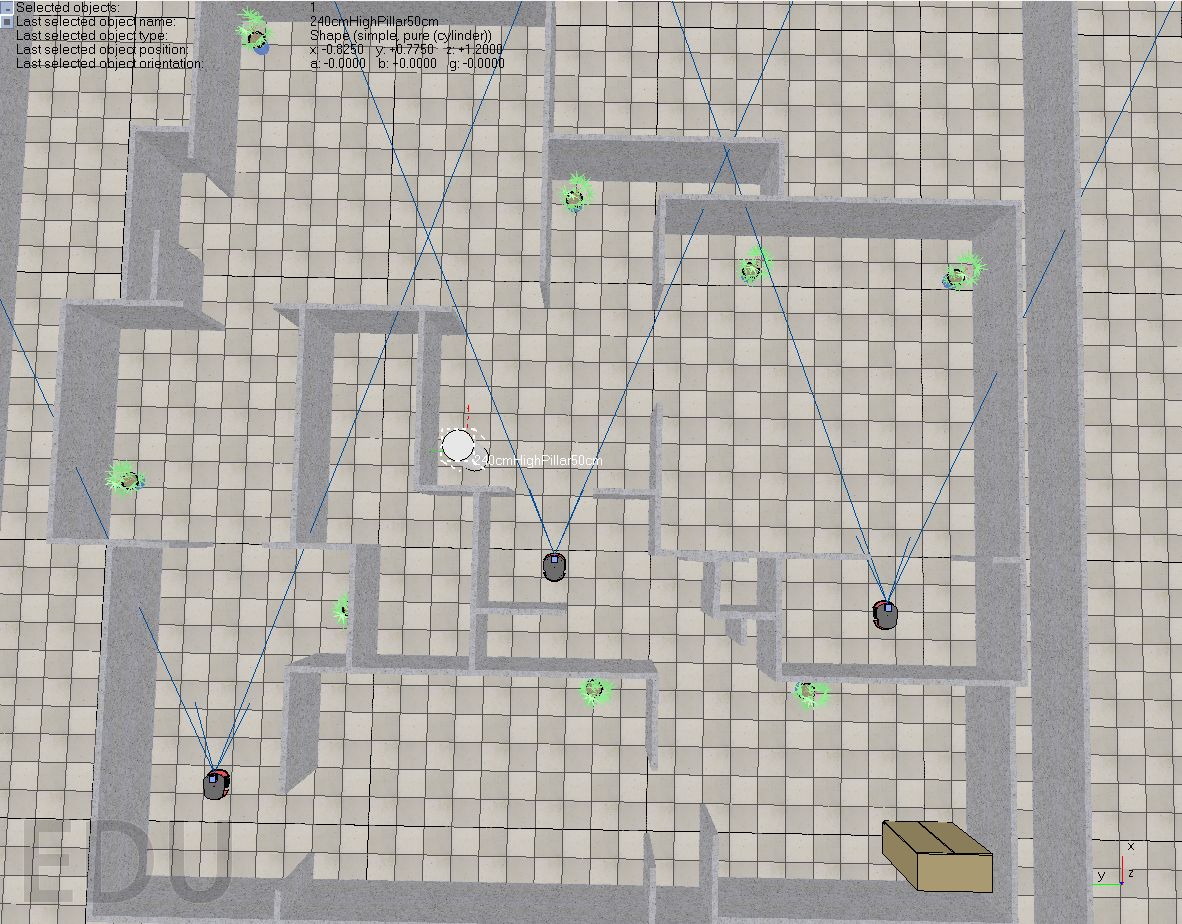
\includegraphics[width=3.93in]{../img/minimal-overlapping-area-scene.png}
    \caption[Scene for experiment with $3$ robots.]{Scene for experiment with $3$ robots in \gls{VREP} simulator. Robot positions in scene are used as initial positions of robots for experiment.}
    \label{fig:minimal-overlapping-area-scene}
\end{figure}

\begin{figure}
    \centering
    % 3.35in
    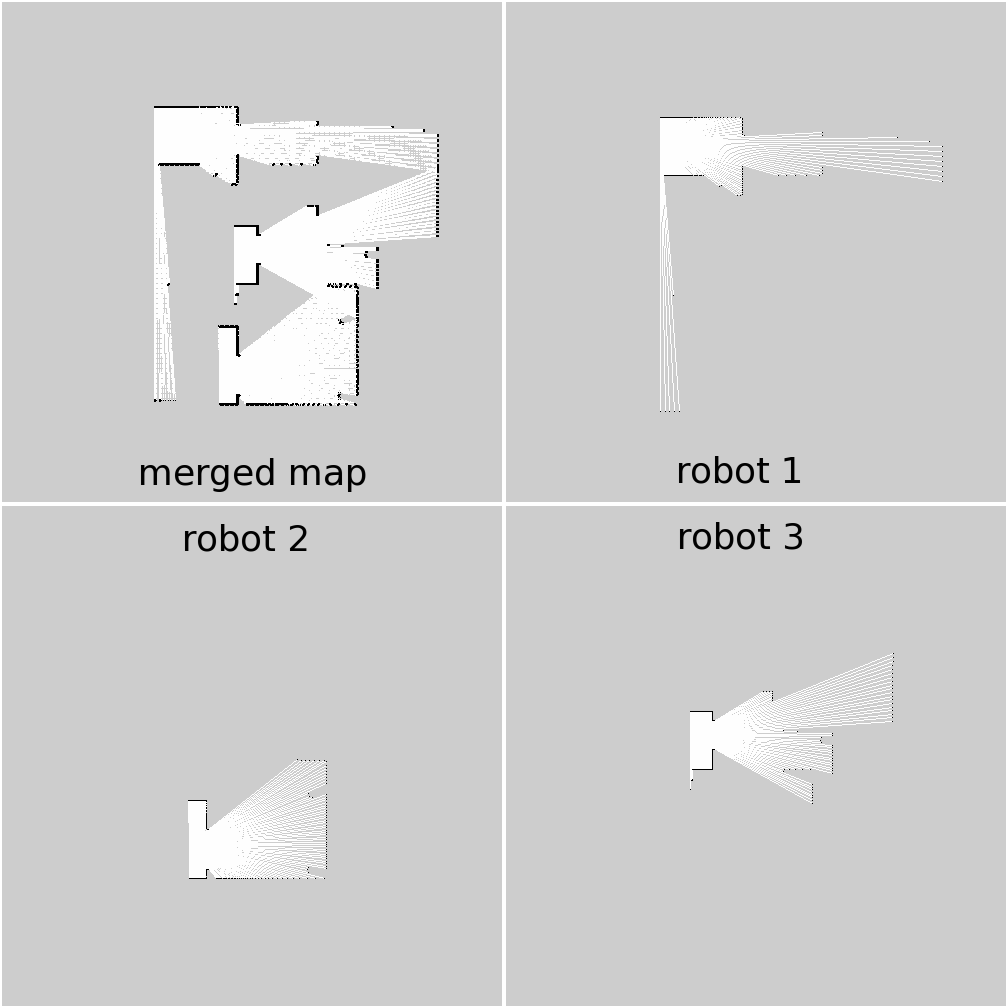
\includegraphics[width=\textwidth]{../img/merging-with-known-initial-positions-begin.png}
    \caption[Initial maps produced by robots in the simulator.]{Initial maps produced by robots during experiment in the simulator. Merged map is produced with knowledge of initial positions and can be therefore produced even without overlapping areas. In this situation merged map can be sparse.}
    \label{fig:merging-with-known-initial-positions-begin}
\end{figure}

\begin{figure}
    \centering
    % 3.35in for 300 dpi
    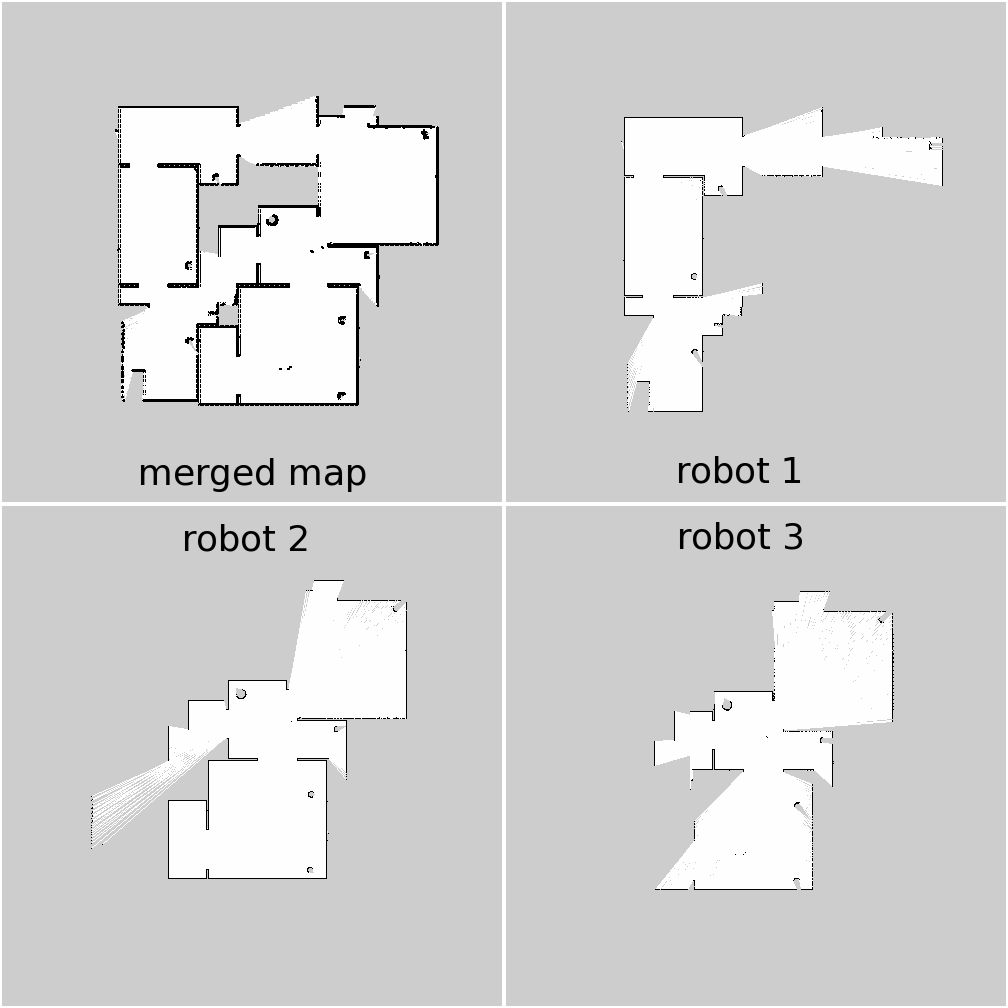
\includegraphics[width=\textwidth]{../img/merging-with-known-initial-positions-end.png}
    \caption[Final maps produced in during experiment the simulator.]{Final maps produced in the simulator. Merged map is produced with knowledge of initial positions.}
    \label{fig:merging-with-known-initial-positions-end}
\end{figure}

\section{Minimal overlapping area}
\label{sec:minimal-overlaping-area}

Map-merging algorithm presented in Section~\ref{chap:mergingalgorithm} relies on overlapping areas of occupancy grids to produce a merged map. Minimal overlapping area to produce a reliable merge depends on environment being explored. Areas with high number of features in occupancy grids require small overlaps and vice versa.

Experiments showed that a reliable merge requires only about $90$ inliers, sometimes only $80$ inliers is enough to produce a correct transformation as seen in Figure~\ref{fig:minimal-overlapping-area-log}. This excerpt is from the log of map-merging node presented in Section~\ref{sec:map_merge-package} acquired during simulation.

Full log containing number of matches and number of inliers required to produce a transformation along with other details is available in the attachments. Scene for \gls{VREP} simulator, merged map and maps produced by robots are also attached. Maps has been taken as screenshots in rviz visualiser.

\begin{figure}
    \centering
	\begin{code}
AffineMatcher: have 121 matches
estimate:
[1.002576035215622, 0.00299917716022613, 62.49276756175958;
 -0.00299917716022613, 1.002576035215622, -240.2015971108993]
num_inliers 83
AffineMatcher: have 147 matches
estimate:
[1.002175802299877, -0.0004136975345276905, -15.26120294301828;
 0.0004136975345276905, 1.002175802299877, -120.7595895934327]
num_inliers 95
AffineMatcher: have 193 matches
estimate:
[1.000933706668138, 0.001232315845354937, 78.01218357952351;
 -0.001232315845354937, 1.000933706668138, -119.6792960984003]
num_inliers 157
	\end{code}
    \caption[Excerpt from the attached log of the map-merging node.]{Excerpt from the attached log of the map-merging node captured during simulation. Shows output of matching phase of the algorithm for $3$ pairwise matches along with number of inliers.}
    \label{fig:minimal-overlapping-area-log}
\end{figure}


Simulation featured $3$ robots exploring common area. Figure~\ref{fig:minimal-overlapping-area-scene} shows the scene used in the experiment and initial robots positions. Figure~\ref{fig:minimal-overlapping-area-final-maps} shows maps produced by \gls{SLAM} and the merged map produced by a map-merging node with unknown initial positions after mapping finished.

Simulation showed that a reliable merge between maps can be produced for $5-6$ overlapping rooms. After transformation is estimated, produced map is comparable to the reference map.

\begin{figure}
    \centering
    % 2.22in for 300dpi
    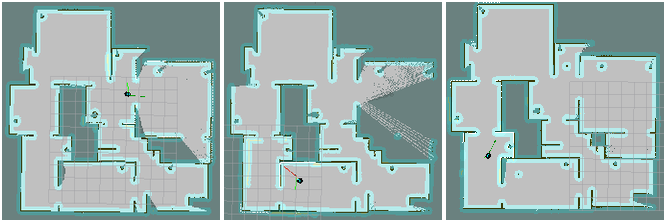
\includegraphics[width=4.44in]{../img/minimal-overlapping-area-final-maps.png}
    \caption[Maps produced by a multi-robot mapping in the simulator.]{Maps produced by a multi-robot mapping in the simulator with $3$ robots. The merged map (bottom right) is estimated by the map-merging node without knowledge of initial positions. Simulated scene can be seen in Figure~\ref{fig:minimal-overlapping-area-scene}. Positions of the robots are final positions where robots finished mapping.}
    \label{fig:minimal-overlapping-area-final-maps}
\end{figure}

\section{Retaining largest transformation}
\label{sec:retaining-largest-transformation}

During online merging the merging algorithm presented in Section~\ref{chap:mergingalgorithm} is launched repeatedly on growing grids. It might seem natural to preserve the transformation between largest number of grids. If the algorithm was able to produce a merge between $n$ grids in one point of time, it might seem like a good idea to preserve this transformation and use it for merging grids when the transformation is estimated for less than $n$ grids.

Experiments showed that this approach produce worse results than approach always using the newest transformation. Largest transformation retaining behaviour is problematic when there is not enough overlapping area between grids. Experiment presented in Section~\ref{sec:merging-with-known-initial-positions} have maps that have very small overlaps.

Map-merging with unknown initial positions with largest transformation retaining launched in the same experiment as presented in Section~\ref{sec:merging-with-known-initial-positions} shows the key problem of a such approach. Problem occurs when incorrect merge is produced due to too small overlaps. As shown in Figure~\ref{fig:retaining-largest-transformation-montage}, incorrect unstable transformations, which are usually corrected quickly with small maps changes, are preserved due to largest transformation retaining after the estimation algorithm is no longer producing incorrect transformation. Incorrect transformations can be preserved for a long period of time with largest transformation retaining behaviour, when there is not enough overlapping area in the maps, so the incorrect transformation can be replaced with correct larger transformation.

Based on this and others experiments largest transformation retaining behaviour has been removed from map-merging node presented in Section~\ref{sec:map_merge-package}.

Data for this experiment including rosbag with map topics, scene for \gls{VREP} simulator and presented maps is available in the attachments.

\begin{figure}
    \centering
    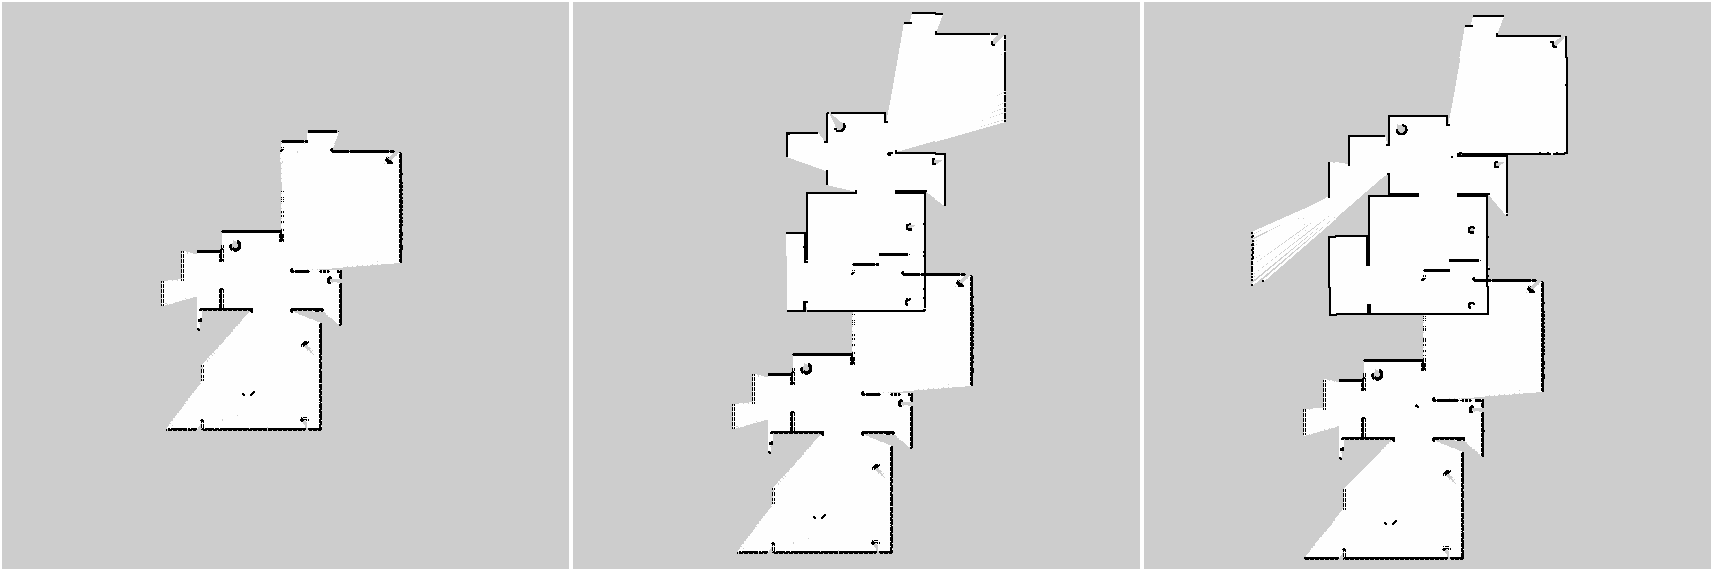
\includegraphics[width=5.71in]{../img/retaining-largest-transformation-montage.png}
    \caption[Map-merging with largest transformation retaining.]{Map-merging with largest transformation retaining. From the left: Maps have no overlaps, unable to merge more than a single map. Incorrect transformation estimated due to too small overlaps. Overlapping space is still too small to produce a merge, but incorrect transformation was rejected. Due to largest transformation retaining incorrect merge is still produced.}
    \label{fig:retaining-largest-transformation-montage}
\end{figure}

\section{Probability model evaluation}
\label{sec:probability-model-evaluation}

Data from \gls{MIT} dataset is complex and difficult for \gls{SLAM} to produce a map without errors. In some cases overlapping areas does not exists. Such data is therefore suitable to test capabilities of map merging node to reject incorrect or non-mergeable maps.

Figure~\ref{fig:probability-model-evaluation-montage} shows $36$ maps obtained from \gls{MIT} dataset, all of them are from second floor. Empty maps are caused by \gls{SLAM} node failure. Note that maps contain many errors, some of them are completely broken as \gls{SLAM} localization failed. \texttt{hector\_slam} node uses only scans from base-mounted laser, better results might be achieved with different \gls{SLAM} approaches using stereo cameras and 3D scanning.

This dataset is very difficult to merge properly, because most of the maps are broken. It is possible to filtrate broken maps from merge, because the area where mapping failed should not match any other maps, but this is very difficult when most of the maps are broken. Furthermore broken maps tend to have more features than correct maps of the same area, these features than may cause invalid matches between two broken maps to be generated making rejecting broken maps even more difficult.

\begin{figure}
    \centering
    \includegraphics[width=\textwidth]{../img/mit-dataset-montage.png}
    \caption[$36$ maps created by \texttt{hector\_slam} from \gls{MIT} dataset.]{$36$ maps created by \texttt{hector\_slam} from \gls{MIT} dataset. Note that the most of the maps contain serious mapping errors. These errors usually comes from \gls{SLAM} invalid estimation of rotation, generating misaligned walls and corners. Because of the new walls and corners, broken maps tend to have more features, especially in broken areas, making filtering of broken maps hard.}
    \label{fig:probability-model-evaluation-montage}
\end{figure}

Merging algorithm uses thresholding described in Section~\ref{sec:findinglargestconnectedcomponent} based on probabilistic model to reject low-confident matches. I have experimented with confidence threshold, which directly affects which matches will be present in merging (matches with low confidence are not considered). Figures~\ref{fig:probability-model-evaluation-treshold_1.0-12maps}, \ref{fig:probability-model-evaluation-treshold_1.5-9maps} and \ref{fig:probability-model-evaluation-treshold_2.0-3maps} show maps merged with confidence thresholds $1.0$, $1.5$ and $2.0$ respectively. Note that number of maps included in the merged map goes from $12$ to $3$.

Experiment has showed that increasing the confidence threshold to values greater that $1.0$ may lead to better results when maps are difficult to merge. Increasing threshold decreases number of maps merged significantly.

Data used for this experiment are available in the attachments. This data consist of maps produced by \gls{SLAM} on \gls{MIT} dataset and merged maps for tested thresholds. Raw data of \gls{MIT} dataset are available online~\cite{Fallon2013}.

\begin{figure}
    \centering
    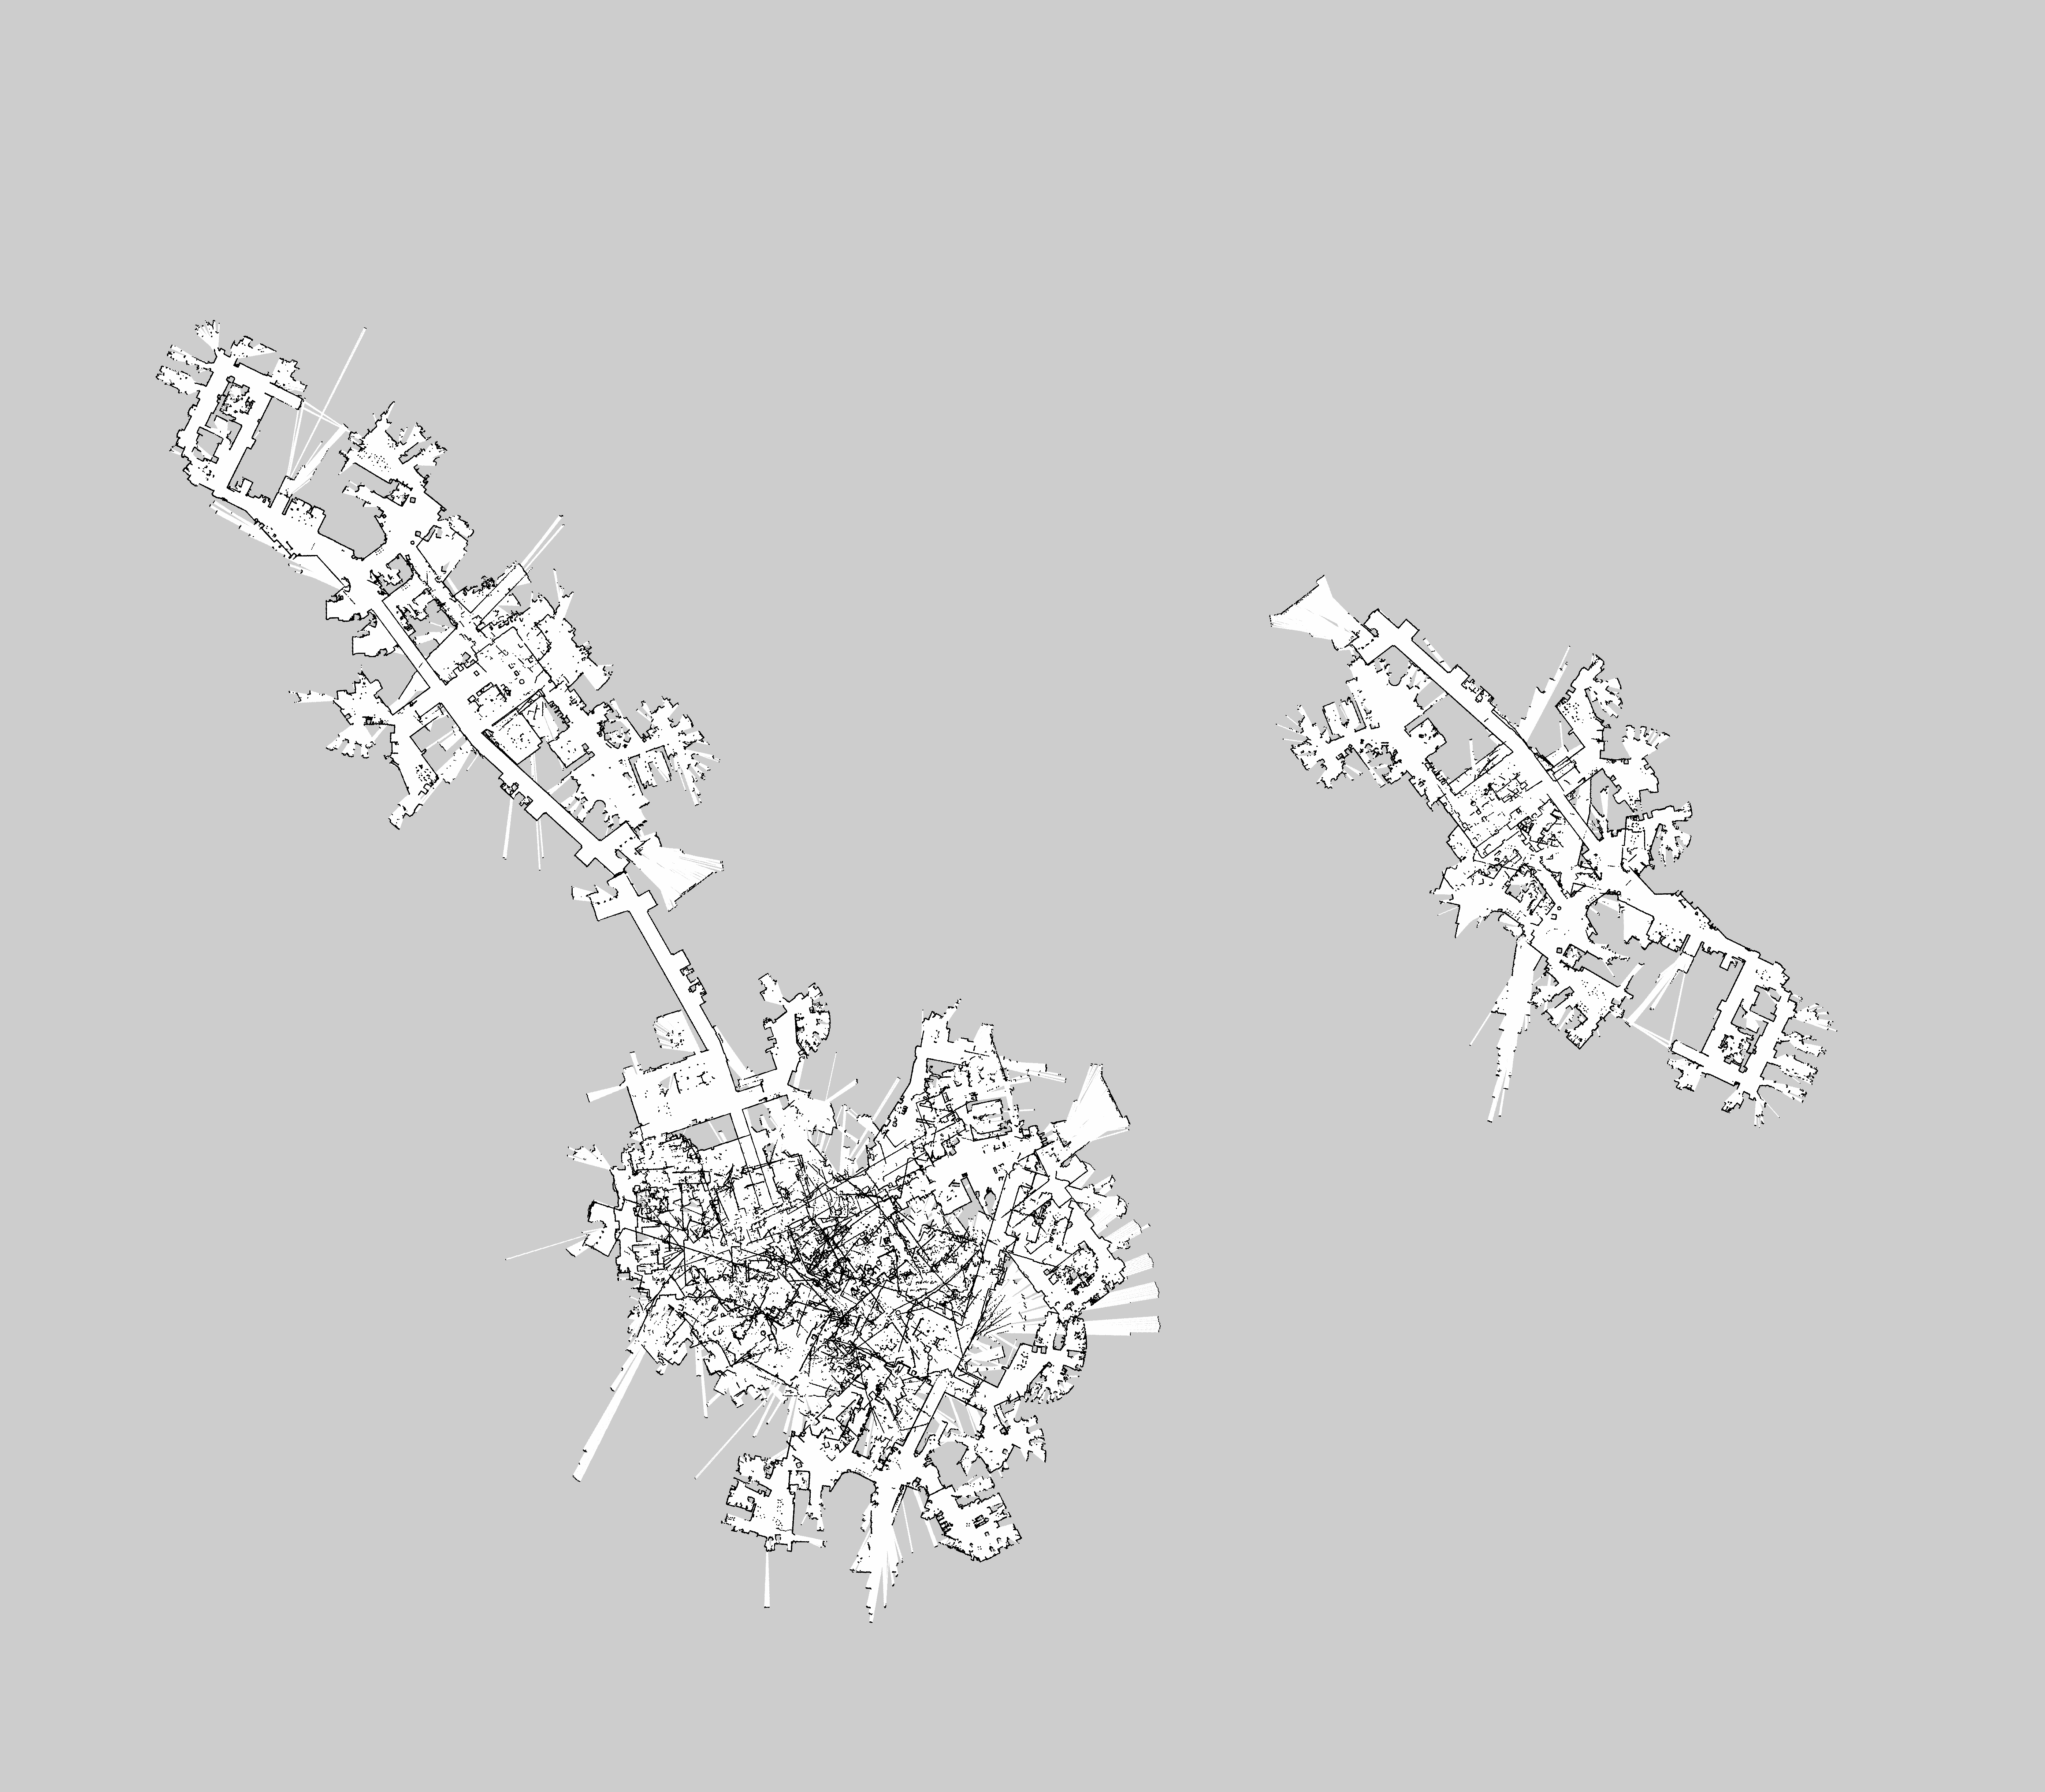
\includegraphics[width=\textwidth]{../img/probability-model-evaluation-treshold_1_0-12maps.png}
    \caption[The merged map created with confidence threshold $1.0$.]{Merged map created from $36$ maps shown in Figure~\ref{fig:probability-model-evaluation-montage}. $12$ maps are included in the merged map. Confidence threshold is set to $1.0$. Although the map-merging algorithm was able to reject $24$ maps, the merged map still includes severely broken maps. Broken areas are feature-rich and thus a wrong transformation is estimated.}
    \label{fig:probability-model-evaluation-treshold_1.0-12maps}
\end{figure}
\begin{figure}
    \centering
    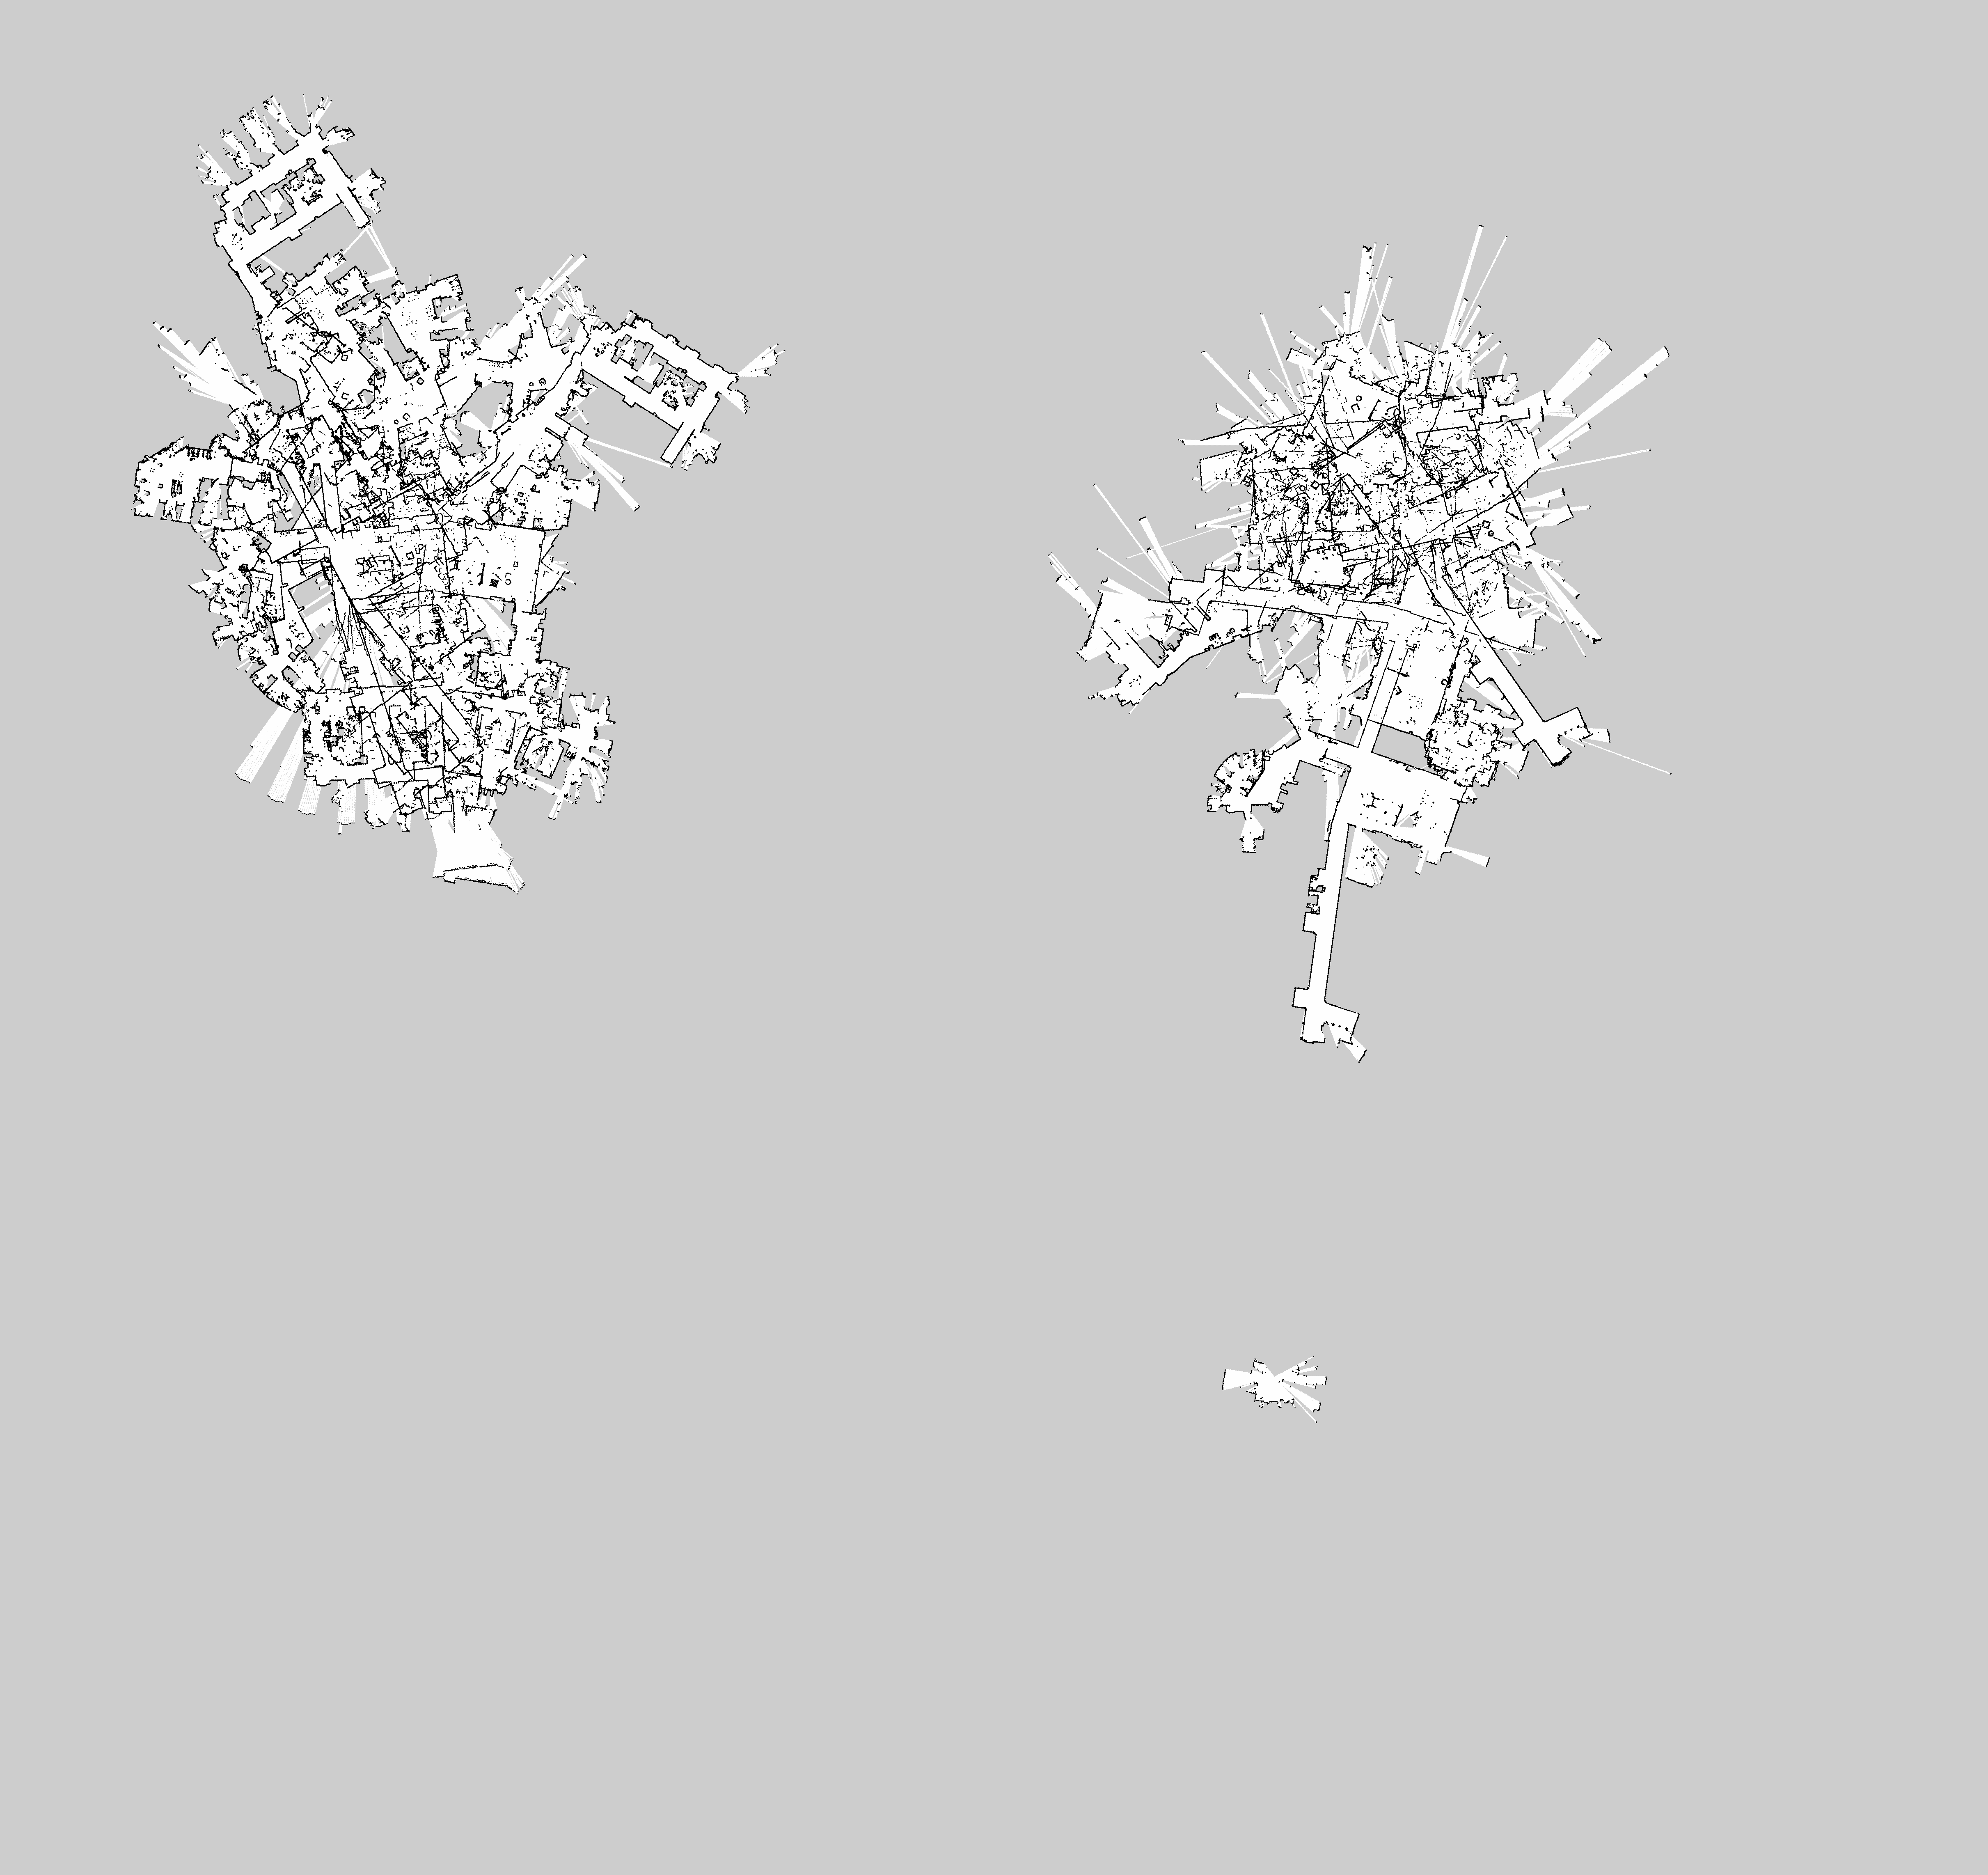
\includegraphics[width=\textwidth]{../img/probability-model-evaluation-treshold_1_5-9maps.png}
    \caption[The merged map created with confidence threshold $1.5$.]{Merged map created from $36$ maps shown in Figure~\ref{fig:probability-model-evaluation-montage}. $9$ maps are included in the merged map. Confidence threshold is set to $1.5$. This map contains even less maps than Figure~\ref{fig:probability-model-evaluation-treshold_1.0-12maps}, but threshold is not high enough to reject all broken maps. Severely broken maps are still included in the merged map. Broken areas in the maps were matched together. These areas are relatively feature-rich and matches between them has got enough \gls{RANSAC} inliers  to be considered confident enough.}
    \label{fig:probability-model-evaluation-treshold_1.5-9maps}
\end{figure}
\begin{figure}
    \centering
    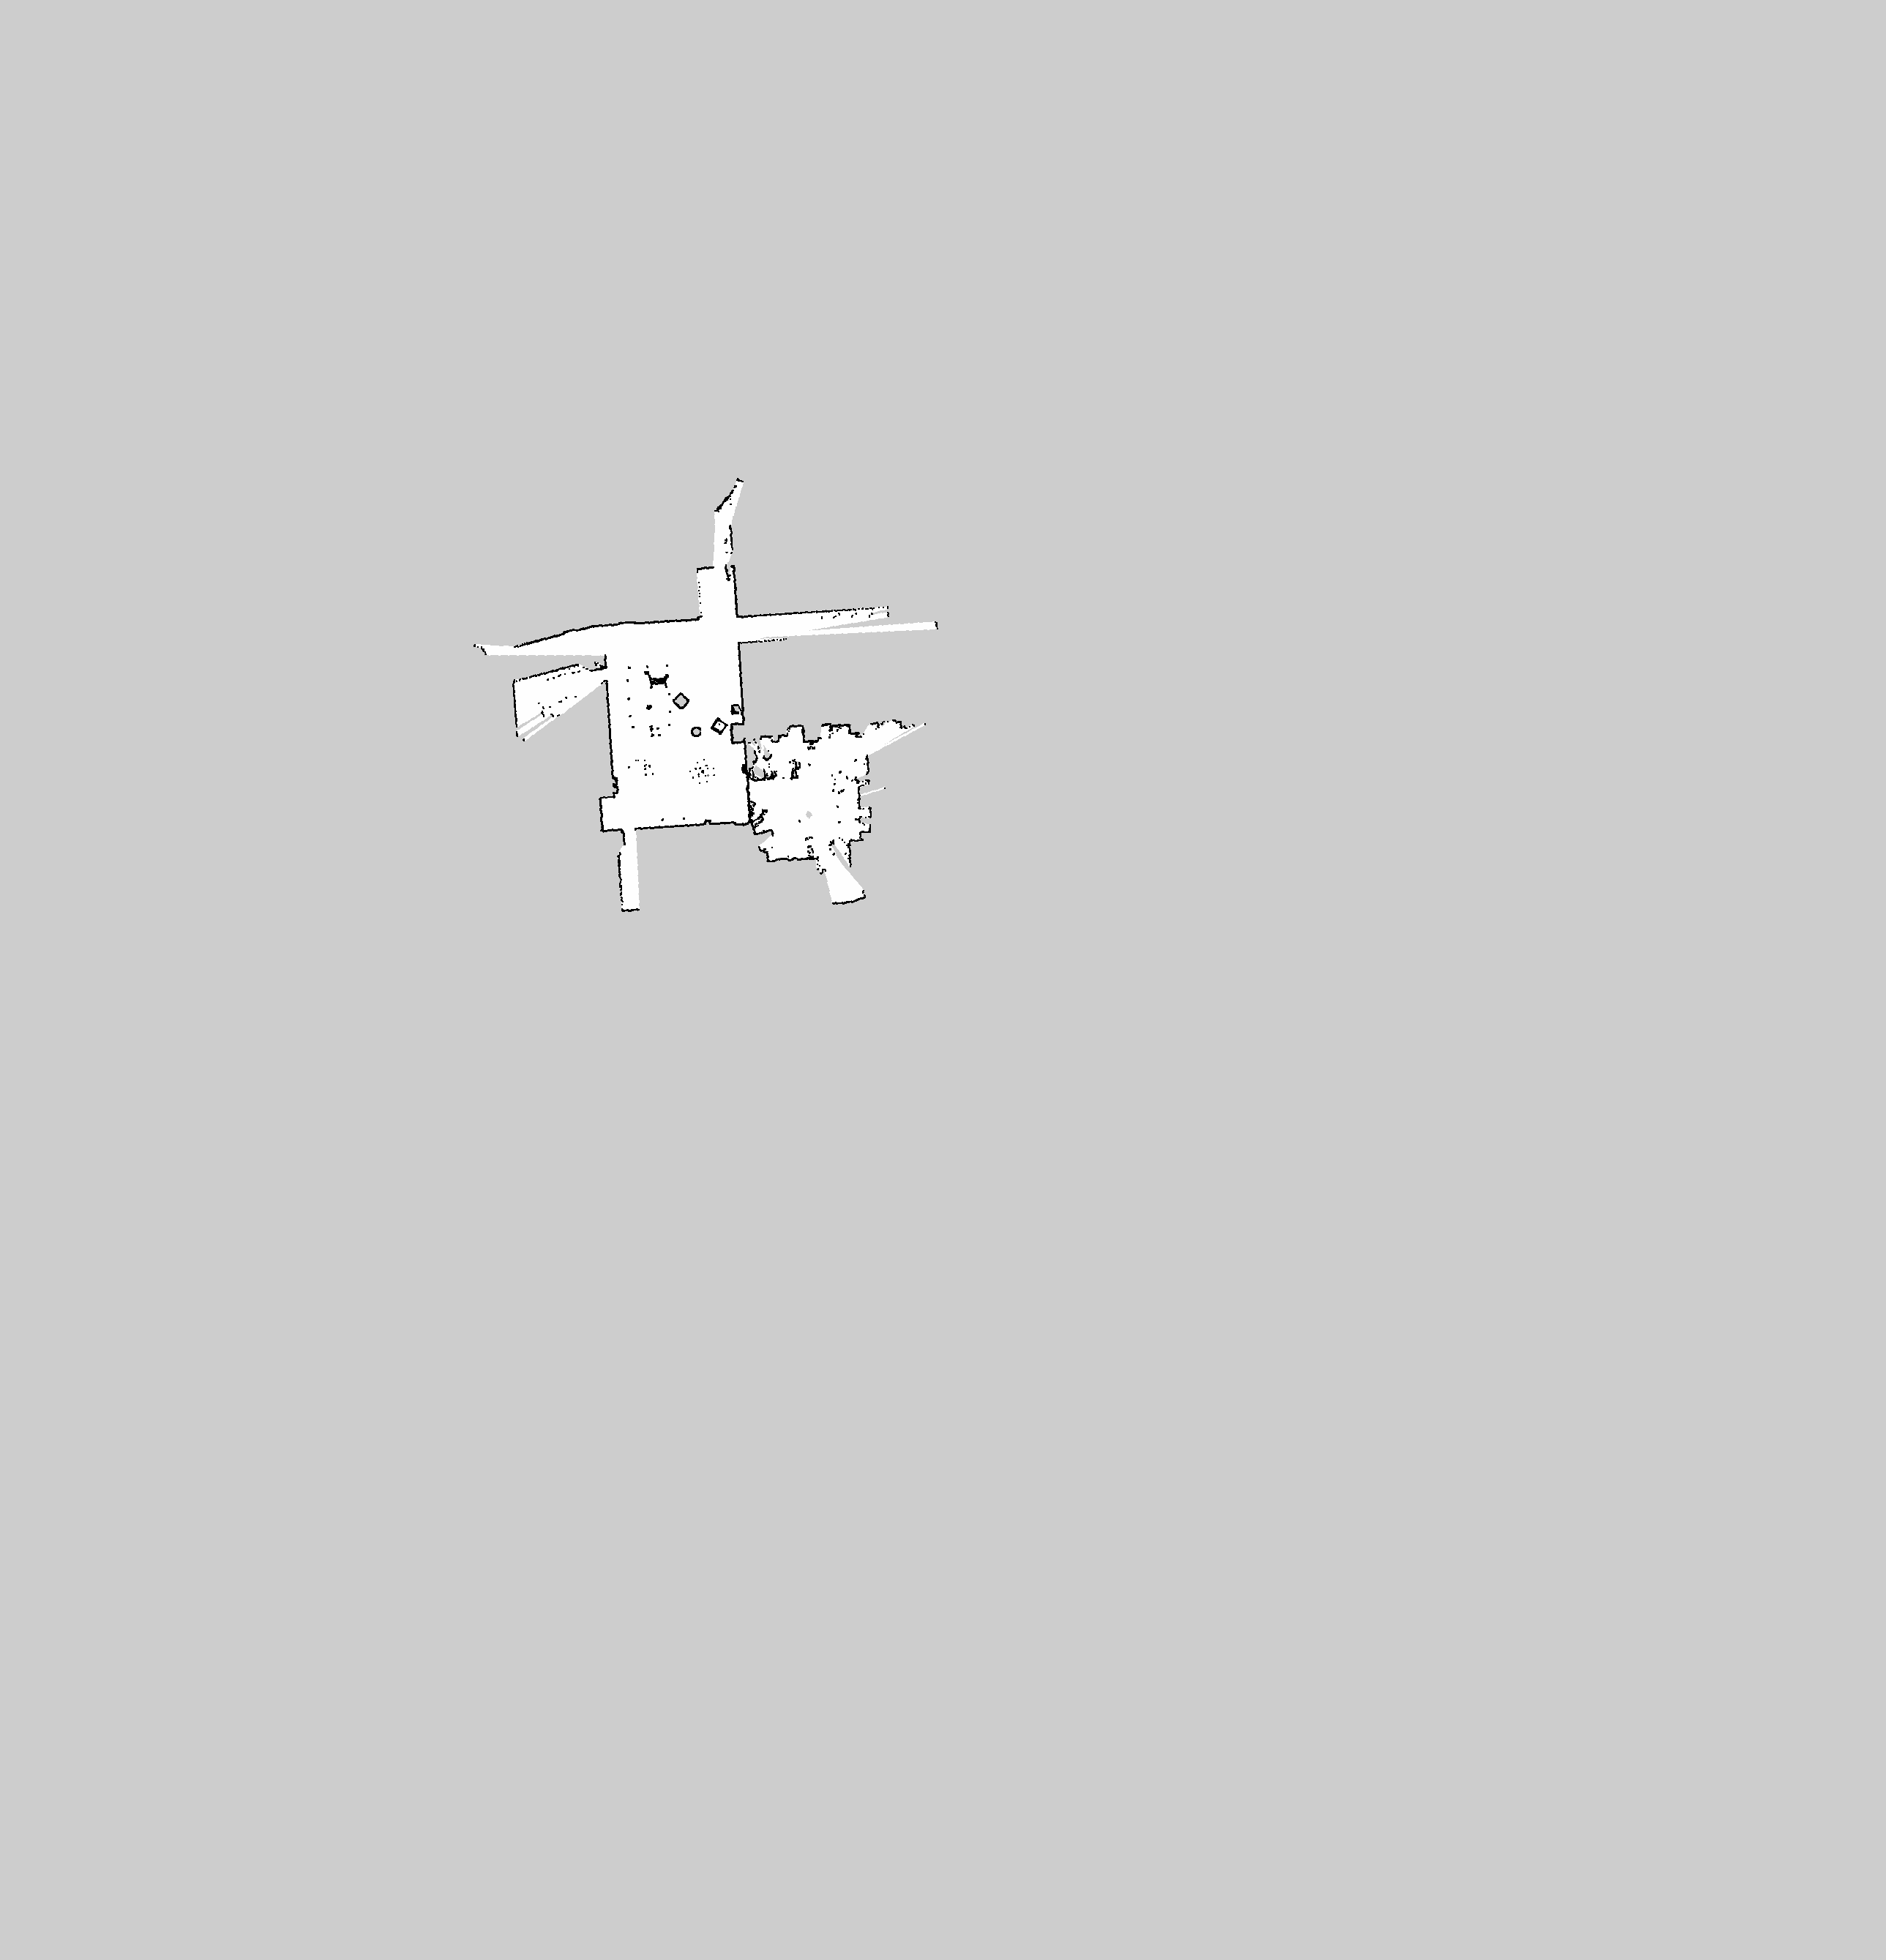
\includegraphics[width=\textwidth]{../img/probability-model-evaluation-treshold_2_0-3maps.png}
    \caption[The merged map created with confidence threshold $2.0$.]{Merged map created from $36$ maps shown in Figure~\ref{fig:probability-model-evaluation-montage}. $3$ maps are included in the merged map. Confidence threshold is set to $2.0$. All broken maps have been rejected. The merged map is correct, transformation between grids was estimated correctly. Maps included in this merged map are small, for larger maps the \gls{SLAM} algorithm mostly failed on presented dataset as seen in Figure~\ref{fig:probability-model-evaluation-montage}.}
    \label{fig:probability-model-evaluation-treshold_2.0-3maps}
\end{figure}

% TODO:
% 3-robots evo 2 - rozbity slam


\chapwithtoc{Conclusion}

Presented map-merging algorithm can efficiently work with artificial number of robots, scales to large multi-robot systems and is designed with parallel processing in mind. Algorithm is suitable for heterogeneous multi-robot teams and is easily deployable with various \gls{SLAM} algorithms.

The algorithm is implemented in \texttt{multirobot\_map\_merge} \gls{ROS} package. This implementation is flexible, poses low requirements on participating robots, does not depend on any particular communication between robots and does not have any presumptions on underlying mechanisms of \gls{SLAM} algorithms used by robots. Those properties allows easy deployment in \gls{ROS} environment for both existing systems and systems build from scratch. Performance of the implemented initial pose estimation algorithm is sufficient to merge map from large number of robots (more than $30$) on a laptop-grade processor. For large number of robots map compositing is the bottleneck for map-merging node, this will be addressed in the next version of the map-merging node.

The map-merging algorithm has been evaluated in the simulation and showed reliable estimates for maps with enough overlapping area. Necessary overlaps range from $5$ to $7$ rooms in a feature-poor simulation. Behaviour for online merging has been studied and implementation has been adapted to produce a consistent map when there is not enough overlapping space.

Evaluation with physical robots is yet to be done. I expect performance for real-world applications to be comparable to the experiments in the simulator or better, because indoor physical environments are usually more feature-rich than scenarios in the simulator. This thesis also focused on map-merging for two-dimensional maps, map-merging for tree-dimensional maps remains an open problem in robotics.


%%% Bibliography
%%% Bibliography (literature used as a source)
%%%
%%% We employ bibTeX to construct the bibliography. It processes
%%% citations in the text (e.g., the \cite{...} macro) and looks up
%%% relevant entries in the bibliography.bib file.
%%%
%%% The \bibliographystyle command selects, which style will be used
%%% for references from the text. The argument in curly brackets is
%%% the name of the corresponding style file (*.bst). Both styles
%%% mentioned in this template are included in LaTeX distributions.

\bibliographystyle{plainnat}    %% Author (year)
% \bibliographystyle{unsrt}     %% [number]

\renewcommand{\bibname}{Bibliography}

%%% Generate the bibliography. Beware that if you cited no works,
%%% the empty list will be omitted completely.

\bibliography{bibliography}

%%% If case you prefer to write the bibliography manually (without bibTeX),
%%% you can use the following. Please follow the ISO 690 standard and
%%% citation conventions of your field of research.

% \begin{thebibliography}{99}
%
% \bibitem{lamport94}
%   {\sc Lamport,} Leslie.
%   \emph{\LaTeX: A Document Preparation System}.
%   2nd edition.
%   Massachusetts: Addison Wesley, 1994.
%   ISBN 0-201-52983-1.
%
% \end{thebibliography}


%%% Figures used in the thesis (consider if this is needed)
\listoffigures

%%% Tables used in the thesis (consider if this is needed)
%%% In mathematical theses, it could be better to move the list of tables to the beginning of the thesis.
%\listoftables

%%% Abbreviations used in the thesis, if any, including their explanation
%%% In mathematical theses, it could be better to move the list of abbreviations to the beginning of the thesis.
%\printglossaries[title=List of Abbreviations]
\printglossary[title=List of Abbreviations,type=\acronymtype]
%\chapwithtoc{List of Abbreviations}

\chapwithtoc{List of Attached Files}
\label{chap:files}

This is a list of files attached to this thesis. Source code is also available online, see appendices~\ref{chap:map_merge-doc}~\ref{chap:explore-doc}.

\medskip
\dirtree{%
.1 attachements.zip. %
.2 merging-with-known-initial-positions\DTcomment{experiment data, see~\ref{sec:merging-with-known-initial-positions}}. %
.2 minimal-overlapping-area\DTcomment{experiment data, see~\ref{sec:minimal-overlaping-area}}. %
.2 retaining-largest-transformation\DTcomment{experiment data, see~\ref{sec:retaining-largest-transformation}}. %
.2 probability-model-evaluation\DTcomment{experiment data, see~\ref{sec:probability-model-evaluation}}. %
.2 m-explore\DTcomment{source code for ROS packages, see~\ref{chap:ros-packages}}. %
.3 explore\DTcomment{see~\ref{sec:explore_lite-package}}. %
.4 doc\DTcomment{package and code documentation}. %
.4 include. %
.5 explore. %
.6 explore.h\DTcomment{ROS node}. %
.6 navfn\_ros.h\DTcomment{ROS planner with extended API, see~\ref{sec:frontier-search}}. %
.6 explore\_frontier.h\DTcomment{see~\ref{sec:frontier-search}}. %
.6 costmap\_client.h\DTcomment{see~\ref{sec:map-sourcing}}. %
.4 launch. %
.4 src. %
.3 map\_merge\DTcomment{see~\ref{sec:map_merge-package}}. %
.4 doc\DTcomment{package and code documentation}. %
.4 test\DTcomment{gtest based tests}. %
.4 include. %
.5 combine\_grids\DTcomment{implements algorithm presented in section~\ref{chap:mergingalgorithm}}. %
.5 occupancy\_grid\_utils\DTcomment{see~\ref{sec:map-composition}}. %
.5 map\_merge. %
.6 map\_merge.h\DTcomment{ROS node}. %
.4 launch. %
.4 src. %
}


%%% Attachments to the bachelor thesis, if any. Each attachment must be
%%% referred to at least once from the text of the thesis. Attachments
%%% are numbered.
%%%
%%% The printed version should preferably contain attachments, which can be
%%% read (additional tables and charts, supplementary text, examples of
%%% program output, etc.). The electronic version is more suited for attachments
%%% which will likely be used in an electronic form rather than read (program
%%% source code, data files, interactive charts, etc.). Electronic attachments
%%% should be uploaded to SIS and optionally also included in the thesis on a~CD/DVD.
%\chapwithtoc{Attachments}
\begin{appendices}
\chapter{multirobot\_map\_merge}
\label{chap:map_merge-doc}

\section{Package Summary}

Merging multiple maps with knowledge of the initial relative positions of robots.

\begin{itemize}
    \item Maintainer status: developed
    \item Maintainer: Jiri Horner \textless laeqten AT gmail DOT com\textgreater
    \item Author: Jiri Horner \textless laeqten AT gmail DOT com\textgreater
    \item License: BSD
    \item Source: git \url{https://github.com/hrnr/m-explore.git} (branch: master)
\end{itemize}

\section{Overview}

This package provides global map for multiple robots. It can merge maps from arbitrary number of robots. It expects maps from individual robots as ROS topics. If your run multiple robots under the same ROS master then \texttt{multirobot\_map\_merge} will probably work for you out-of-the-box. It is also very easy to setup an simulation experiment.

\begin{figure}
    \centering
    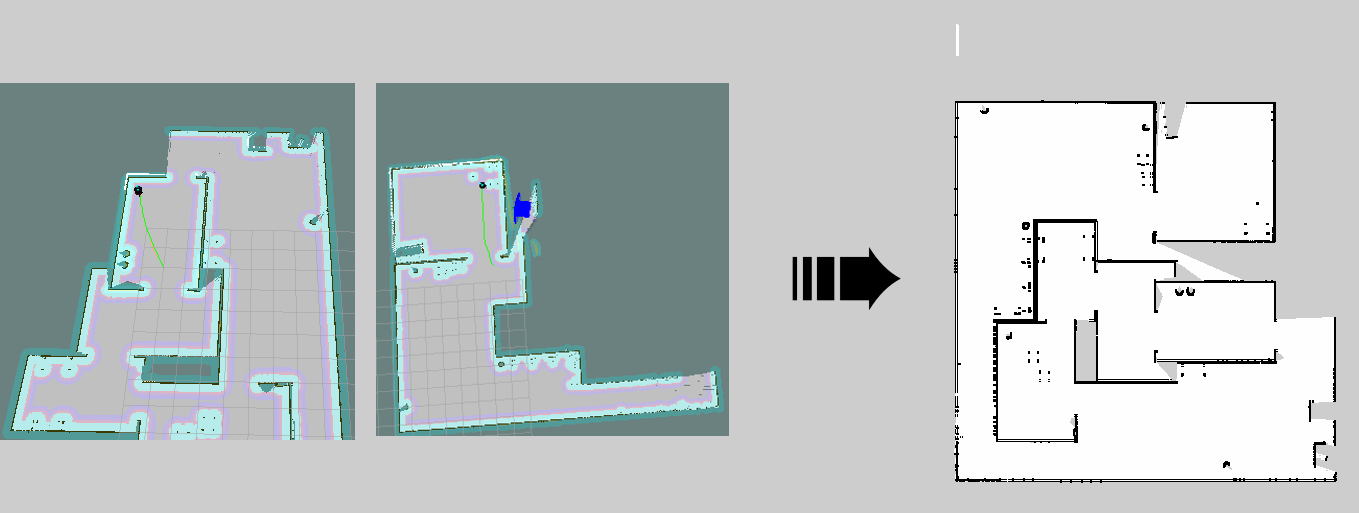
\includegraphics[width=4.53in]{../img/map_merge_cover.png}
    \caption{Output of \texttt{multirobot\_map\_merge}, map merging node for \gls{ROS}. Merged map from $2$ robots. Robots in the environment visualised on the left, merged map on the right.}
    \label{fig:mapmergecover}
\end{figure}

If your run your robots under multiple ROS masters you need to run your own way of communication between robots and provide maps from robots on local topics (under the same master). Also if you want to distribute merged map back to robots your communication must take care of it.

%<<Youtube(8Adrn29BVbM&rel=0)>>

\texttt{multirobot\_map\_merge} does not depend on any particular communication between robots.

\section{Architecture}

\texttt{multirobot\_map\_merge} finds robot maps dynamically and new robots can be added to system at any time.

\begin{figure}
    \centering
    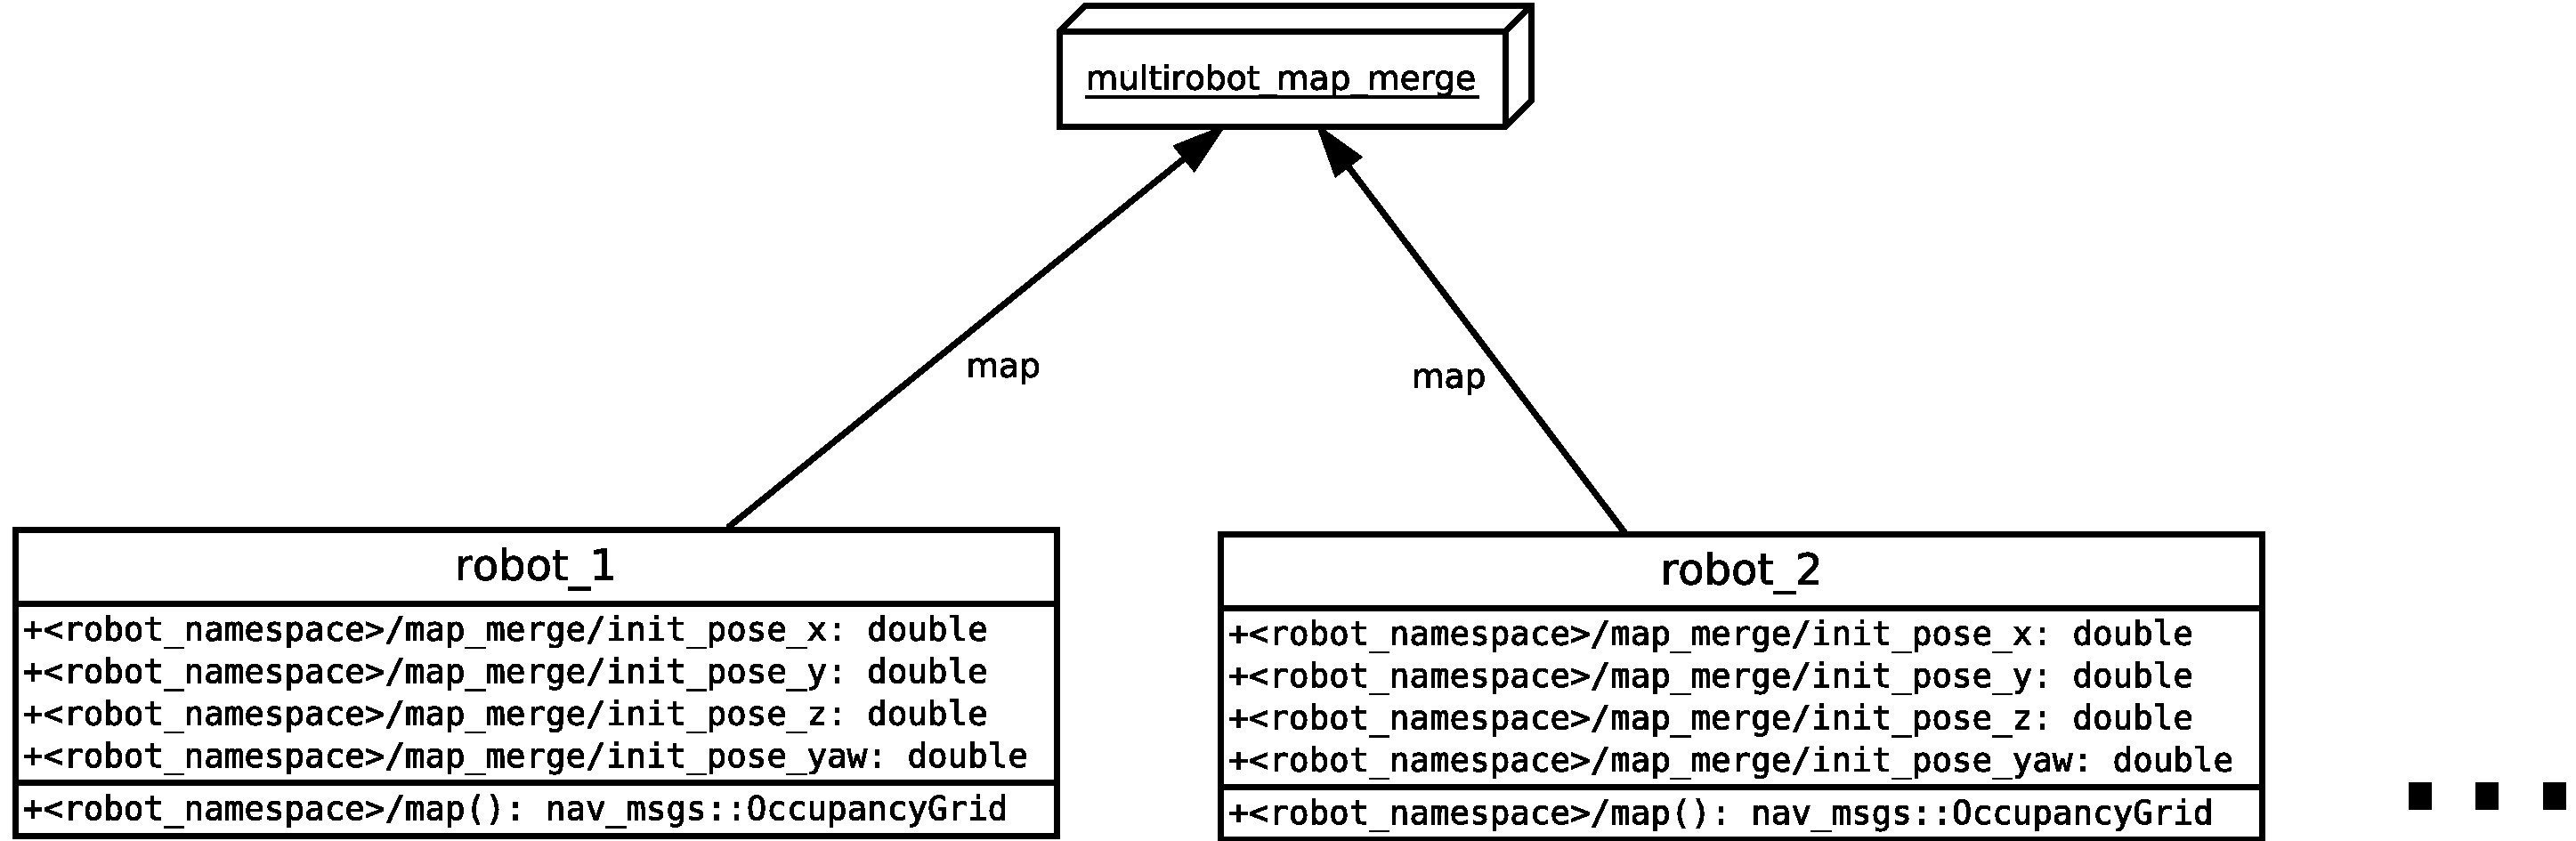
\includegraphics[width=\textwidth]{../img/map_merge_architecture.pdf}
    \caption{Architecture of \texttt{multirobot\_map\_merge}, proposed map merging node for \gls{ROS}.}
    \label{fig:mapmergearchitecture}
\end{figure}

To make this dynamic behaviour possible there are some constrains placed on robots. First all robots must publish map under \texttt{<robot\_namespace>/map}, where topic name (\texttt{map}) is configurable, but must be same for all robots. For each robot \texttt{<robot\_namespace>} will be of cause different.

This node support merging maps with known initial positions of the robots or without. See below for details.

\section{Merging modes}
\label{sec:mergingmodes}

Two merging modes are currently supported as orthogonal options. If you know initial positions of robots you may preferably use the first mode and get exact results (rigid transformation will be computed according to initial positions). If you don't know robot's starting points you are still able to use the second mode where transformation between grids will be determined using heuristic algorithm. You can choose between these two modes using the \texttt{known\_init\_poses} parameter.

\subsection{merging with known initial positions}

This is preferred mode whenever you are able to determine exact starting point for each robot. You need to provide initial position for each robot. You need to provide set of \texttt{<robot\_namespace>/map\_merge/init\_pose} parameters. These positions should be in \texttt{world\_frame}. See~\ref{sec:rosapi}.

In this merging these parameters are mandatory. If any of the required parameters is missing robot won't be considered for merging (you will get warning with name of affected robot).

\subsection{merging without known initial positions}

If you can't provide initial poses for robots this mode has minimal configuration requirements. You need to provide only map topic for each robot. Transformation between grids is estimated by feature-matching algorithm and therefore requires grids to have sufficient amount of overlapping space to make a high-probability match. If grids don't have enough overlapping space to make a solid match, merged map can differ greatly from physical situation.

Estimating transforms between grids is cpu-intesive so you might want to tune \texttt{estimation\_rate} parameter to run re-estimation less often if it causes any troubles.

\section{ROS API}
\label{sec:rosapi}

\subsection{map\_merge}

Provides map merging services offered by this package. Dynamically looks for new robots in the system and merges their maps.

\subsubsection{Subscribed Topics}
  \ROStopic{<robot\_namespace>/map}{nav\_msgs/OccupancyGrid}{Local map for specific robot.}

  \ROStopic{<robot\_namespace>/map\_updates}{map\_msgs/OccupancyGridUpdate}{Local map updates for specific robot. Most of the \texttt{nav\_msgs/OccupancyGrid} sources (mapping algorithms) provides incremental map updates via this topic so they don't need to send always full map. This topic is optional. If your mapping algorithm does not provide this topic it is safe to ignore this topic. However if your mapping algorithm does provide this topic, it is preferable to subscribe to this topic. Otherwise map updates will be slow as all partial updates will be missed and map will be able to update only on full map updates.}

\subsubsection{Published Topics}
  \ROStopic{map}{nav\_msgs/OccupancyGrid}{Merged map from all robots in the system.}

\subsubsection{Parameters}
\paragraph{Robot Parameters}

Parameters that should be defined in the namespace of each robot if you want to use merging with known initial poses of robots (\texttt{known\_init\_poses} is \texttt{true}). Without these parameters robots won't be considered for merging. If you can't provide these parameters use merging without known initial poses. See~\ref{sec:mergingmodes}

    \ROSparam{<robot\_namespace>/map\_merge/init\_pose\_x}{<no\_default>}{double}{\texttt{x} coordinate of robot initial position in \texttt{world\_frame}. Should be in meters. It does not matter which frame you will consider global (preferably it should be different from all robots frames), but relative positions of robots in this frame must be correct.}

    \ROSparam{<robot\_namespace>/map\_merge/init\_pose\_y}{<no\_default>}{double}{\texttt{y} coordinate of robot initial position in \texttt{world\_frame}.}

    \ROSparam{<robot\_namespace>/map\_merge/init\_pose\_z}{<no\_default>}{double}{\texttt{z} coordinate of robot initial position in \texttt{world\_frame}.}

    \ROSparam{<robot\_namespace>/map\_merge/init\_pose\_yaw}{<no\_default>}{double}{\texttt{yaw} component of robot initial position in \texttt{world\_frame}. Represents robot rotation in radians.}

\paragraph{Node Parameters}

Parameters that should be defined in the namespace of this node.

    \ROSparam{\~{}robot\_map\_topic}{map}{string}{Name of robot map topic without namespaces (last component of topic name). Only topics with this name will be considered when looking for new maps to merge. This topics may be subject to further filtering (see below).}

    \ROSparam{\~{}robot\_map\_updates\_topic}{map\_updates}{string}{Name of robot map updates topic of \texttt{map\_msgs/OccupancyGridUpdate} without namespaces (last component of topic name). This topic will be always subscribed in the same namespace as \texttt{robot\_map\_topic}. You'll likely need to change this only when you changed \texttt{robot\_map\_topic}. These topics are never considered when searching for new robots.}

    \ROSparam{\~{}robot\_namespace}{<empty string>}{string}{Fixed part of robot map topic. You can employ this parameter to further limit which topics will be considered during dynamic lookup for robots. Only topics which contain (anywhere) this string will be considered for lookup. Unlike \texttt{robot\_map\_topic} you are not limited by namespace logic. Topics will be filtered using text-based search. Therefore \texttt{robot\_namespace} does not need to be ROS namespace, but can contain slashes etc. This must be common part of all robots map topics name (all robots for which you want to merge map).}

    \ROSparam{\~{}known\_init\_poses}{true}{bool}{Selects between merging modes. \texttt{true} if merging with known initial positions. See~\ref{sec:mergingmodes}}

    \ROSparam{\~{}merged\_map\_topic}{map}{string}{Topic name where merged map will be published.}

    \ROSparam{\~{}world\_frame}{world}{string}{Frame id (in \href{http://wiki.ros.org/tf}{tf} tree) which will be assigned to published merged map. This should be frame where you specified robot initial positions.}

    \ROSparam{\~{}merging\_rate}{4.0}{double}{Rate in Hz. Basic frequency on which this node discovers merges robots maps and publish merged map. Increase this value if you want faster updates.}

    \ROSparam{\~{}discovery\_rate}{0.05}{double}{Rate in Hz. Frequency on which this node discovers new robots. Increase this value if you need more agile behaviour when adding new robots. Robots will be discovered sooner.}

    \ROSparam{\~{}estimation\_rate}{0.5}{double}{Rate in Hz. This parameter is relevant only when merging without known positions, see~\ref{sec:mergingmodes}. Frequency on which this node re-estimates transformation between grids. Estimation is cpu-intensive, so you may wish to lower this value.}

\section{Acknowledgements}

This package was developed as part of my bachelor thesis at \href{http://www.mff.cuni.cz/to.en/}{Charles University} in Prague.

Idea for dynamic robot discovery is from \href{http://wiki.ros.org/map_merging}{map\_merging} package from Zhi Yan. Merging algorithm and configuration are different.

\chapter{explore\_lite}
\label{chap:explore-doc}

\section{Package Summary}

Lightweight frontier-based exploration.

\begin{itemize}
    \item Maintainer status: developed
    \item Maintainer: Jiri Horner \textless laeqten AT gmail DOT com\textgreater
    \item Author: Jiri Horner  \textless laeqten AT gmail DOT com\textgreater
    \item License: BSD
    \item Source: git \url{https://github.com/hrnr/m-explore.git} (branch: master)
\end{itemize}

\section{Overview}

This package provides greedy frontier-based exploration. When node is running, robot will greedily explore its enviroment until no frontiers could be found. Movement commands will be send to \href{http://wiki.ros.org/move_base}{move\_base}.

\begin{figure}
    \centering
    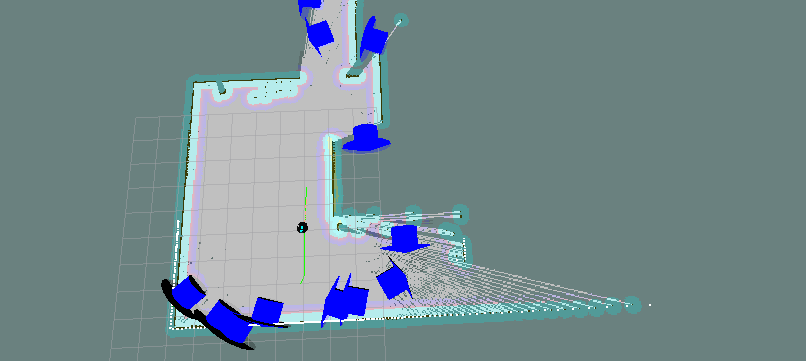
\includegraphics[width=2.68in]{../img/explore_cover.png}
    \caption{Visualisation of robot during exploring. Frontiers found in the map are visualised as blue arrows.}
    \label{fig:explorecover}
\end{figure}

Unlike similar packages, \texttt{explore\_lite} does not create it's own costmap. Node subscribes to \texttt{nav\_msgs/OccupancyGrid} messages. Commands for robot movement are send to \href{http://wiki.ros.org/move_base}{move\_base} node.

\section{Architecture}

\texttt{explore\_lite} uses \href{http://wiki.ros.org/move_base}{move\_base} for navigation. You need to run properly configured \href{http://wiki.ros.org/move_base}{move\_base} node.

\begin{figure}
    \centering
    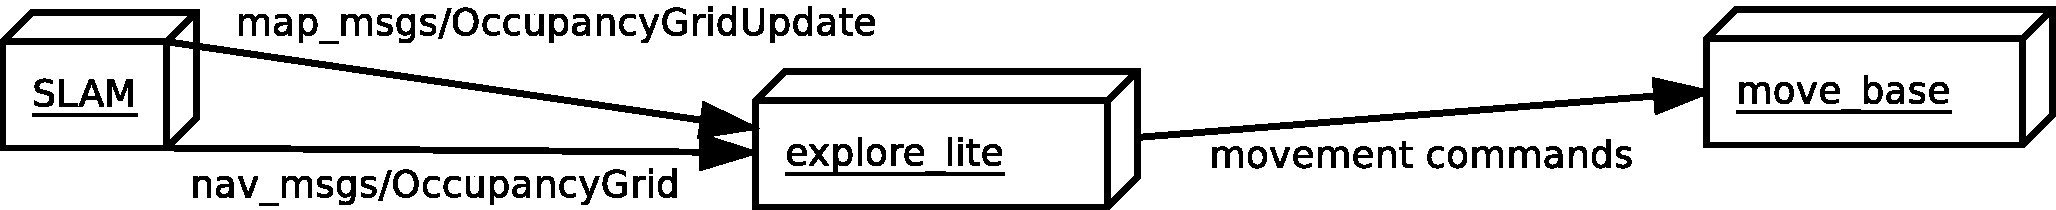
\includegraphics[width=\textwidth]{../img/explore_architecture.pdf}
    \caption{Architecture of \texttt{explore\_lite}, exploring node for \gls{ROS}.}
    \label{fig:explorearchitecture}
\end{figure}

\texttt{explore\_lite} subscribes to a \texttt{nav\_msgs/Occu\-pan\-cy\-Grid} and \texttt{map\_msgs/Occu\-pan\-cy\-Grid\-Up\-da\-te} messages to construct a map where it looks for frontiers. You can either use costmap published by \href{http://wiki.ros.org/move_base}{move\_base} (ie. \texttt{<mo\-ve\_ba\-se>/glo\-bal\_cost\-map/\-cost\-map}) or you can use map constructed by mapping algorithm (SLAM). Better results were achieved on maps constructed by SLAM as they usually contain less noise.

\section{ROS API}
\subsection{explore}

Provides exploration services offered by this package. Exploration will start immediately after node initialization.

\subsubsection{Actions Called}
  \ROStopic{move\_base}{move\_base\_msgs/MoveBaseAction}{\href{http://wiki.ros.org/move_base}{move\_base} actionlib API for posting goals. See \href{http://wiki.ros.org/move_base\#Action_API}{move\_base\#Action API} for details. This expects \href{http://wiki.ros.org/move_base}{move\_base} node in the same namespace as \texttt{explore\_lite}, you may want to remap this node if this is not true.}

\subsubsection{Subscribed Topics}
  \ROStopic{costmap}{nav\_msgs/OccupancyGrid}{Map which will be used for exploration planning. Can be either cost from \href{http://wiki.ros.org/move_base}{move\_base} or map created by SLAM (see above). Occupancy grid must have got properly marked unknown space, mapping algorithms usually track unknown space by default. If you want to use costmap provided by \href{http://wiki.ros.org/move_base}{move\_base} you need to enable unknown space tracking by setting \texttt{track\_unknown\_space: true}.}

  \ROStopic{costmap\_updates}{map\_msgs/OccupancyGridUpdate}{Incremental updates on costmap. Not necessary if source of map is always publishing full updates, i.e. does not provide this topic.}

\subsubsection{Published Topics}
  \ROStopic{\~{}frontiers}{visualization\_msgs/MarkerArray}{Visualization of frontiers considered by exploring algorithm. Each frontier is visualized as vector in the middle of frontier pointing towards unknown area.}

\subsubsection{Parameters}
  \ROSparam{\~{}robot\_base\_frame}{base\_link}{string}{The name of the base frame of the robot. This is used for determining robot position on map. Mandatory.}

  \ROSparam{\~{}costmap\_topic}{costmap}{string}{Specifies topic of source \texttt{nav\_msgs/OccupancyGrid}. Mandatory.}

  \ROSparam{\~{}costmap\_updates\_topic}{costmap\_updates}{string}{Specifies topic of source \texttt{map\_msgs/OccupancyGridUpdate}. Not necessary if source of map is always publishing full updates, i.e. does not provide this topic.}

  \ROSparam{\~{}visualize}{false}{bool}{Specifies whether or not publish visualized frontiers.}

  \ROSparam{\~{}planner\_frequency}{1.0}{double}{Rate in Hz at which new frontiers will computed and goal reconsidered.}

  \ROSparam{\~{}progress\_timeout}{30.0}{double}{Time in seconds. When robot do not make any progress for \texttt{progress\_timeout}, current goal will be abandoned.}

  \ROSparam{\~{}potential\_scale}{1e-3}{double}{Used for weighting frontiers. This multiplicative parameter affects frontier potential component of the frontier weight.}

  \ROSparam{\~{}orientation\_scale}{0}{double}{Used for weighting frontiers. This multiplicative parameter affects frontier orientation component of the frontier weight.}

  \ROSparam{\~{}gain\_scale}{1.0}{double}{Used for weighting frontiers. This multiplicative parameter affects frontier gain component of the frontier weight.}

  \ROSparam{\~{}transform\_tolerance}{0.3}{double}{Transform tolerance to use when transforming robot pose.}

\subsubsection{Required tf Transforms}
  \ROStransform{global\_frame}{robot\_base\_frame}{This transformation is usually provided by mapping algorithm. Those frames are usually called \texttt{map} and \texttt{base\_link}. For adjusting \texttt{robot\_base\_frame} name see respective parameter. You don't need to set \texttt{global\_frame}. The name for \texttt{global\_frame} will be sourced from \texttt{costmap\_topic} automatically.}

\section{Acknowledgements}

This package was developed as part of my bachelor thesis at \href{http://www.mff.cuni.cz/to.en/}{Charles University} in Prague.

This project uses parts of frontier exploration algorithm from \href{http://wiki.ros.org/explore}{explore} package by Charles DuHadway.

\end{appendices}

\openright
\end{document}
